%==============================================================================
% tento soubor pouzijte jako zaklad
% this file should be used as a base for the thesis
% Autoři / Authors: 2008 Michal Bidlo, 2019 Jaroslav Dytrych
% Kontakt pro dotazy a připomínky: sablona@fit.vutbr.cz
% Contact for questions and comments: sablona@fit.vutbr.cz
%==============================================================================
% kodovani: UTF-8 (zmena prikazem iconv, recode nebo cstocs)
% encoding: UTF-8 (you can change it by command iconv, recode or cstocs)
%------------------------------------------------------------------------------
% zpracování / processing: make, make pdf, make clean
%==============================================================================
% Soubory, které je nutné upravit nebo smazat: / Files which have to be edited or deleted:
%   projekt-20-literatura-bibliography.bib - literatura / bibliography
%   projekt-01-kapitoly-chapters.tex - obsah práce / the thesis content
%   projekt-01-kapitoly-chapters-en.tex - obsah práce v angličtině / the thesis content in English
%   projekt-30-prilohy-appendices.tex - přílohy / appendices
%   projekt-30-prilohy-appendices-en.tex - přílohy v angličtině / appendices in English
%==============================================================================
%\documentclass[]{fitthesis} % bez zadání - pro začátek práce, aby nebyl problém s překladem
%\documentclass[english]{fitthesis} % without assignment - for the work start to avoid compilation problem
\documentclass[zadani]{fitthesis} % odevzdani do wisu a/nebo tisk s barevnými odkazy - odkazy jsou barevné
%\documentclass[english,zadani]{fitthesis} % for submission to the IS FIT and/or print with color links - links are color
%\documentclass[zadani,print]{fitthesis} % pro černobílý tisk - odkazy jsou černé
%\documentclass[english,zadani,print]{fitthesis} % for the black and white print - links are black
%\documentclass[zadani,cprint]{fitthesis} % pro barevný tisk - odkazy jsou černé, znak VUT barevný
%\documentclass[english,zadani,cprint]{fitthesis} % for the print - links are black, logo is color
% * Je-li práce psaná v anglickém jazyce, je zapotřebí u třídy použít 
%   parametr english následovně:
%   If thesis is written in English, it is necessary to use 
%   parameter english as follows:
%      \documentclass[english]{fitthesis}
% * Je-li práce psaná ve slovenském jazyce, je zapotřebí u třídy použít 
%   parametr slovak následovně:
%   If the work is written in the Slovak language, it is necessary 
%   to use parameter slovak as follows:
%      \documentclass[slovak]{fitthesis}
% * Je-li práce psaná v anglickém jazyce se slovenským abstraktem apod., 
%   je zapotřebí u třídy použít parametry english a enslovak následovně:
%   If the work is written in English with the Slovak abstract, etc., 
%   it is necessary to use parameters english and enslovak as follows:
%      \documentclass[english,enslovak]{fitthesis}

% Základní balíčky jsou dole v souboru šablony fitthesis.cls
% Basic packages are at the bottom of template file fitthesis.cls
% zde můžeme vložit vlastní balíčky / you can place own packages here

% Kompilace po částech (rychlejší, ale v náhledu nemusí být vše aktuální)
% Compilation piecewise (faster, but not all parts in preview will be up-to-date)
% \usepackage{subfiles}

% Nastavení cesty k obrázkům
% Setting of a path to the pictures
%\graphicspath{{obrazky-figures/}{./obrazky-figures/}}
%\graphicspath{{obrazky-figures/}{../obrazky-figures/}}

%---rm---------------
\renewcommand{\rmdefault}{lmr}%zavede Latin Modern Roman jako rm / set Latin Modern Roman as rm
%---sf---------------
\renewcommand{\sfdefault}{qhv}%zavede TeX Gyre Heros jako sf
%---tt------------
\renewcommand{\ttdefault}{lmtt}% zavede Latin Modern tt jako tt

% vypne funkci šablony, která automaticky nahrazuje uvozovky,
% aby nebyly prováděny nevhodné náhrady v popisech API apod.
% disables function of the template which replaces quotation marks
% to avoid unnecessary replacements in the API descriptions etc.
\csdoublequotesoff



\usepackage{url}


% my custom usepackages
\usepackage{dirtree}

% =======================================================================
% balíček "hyperref" vytváří klikací odkazy v pdf, pokud tedy použijeme pdflatex
% problém je, že balíček hyperref musí být uveden jako poslední, takže nemůže
% být v šabloně
% "hyperref" package create clickable links in pdf if you are using pdflatex.
% Problem is that this package have to be introduced as the last one so it 
% can not be placed in the template file.
\ifWis
\ifx\pdfoutput\undefined % nejedeme pod pdflatexem / we are not using pdflatex
\else
  \usepackage{color}
  \usepackage[unicode,colorlinks,hyperindex,plainpages=false,pdftex]{hyperref}
  \definecolor{hrcolor-ref}{RGB}{223,52,30}
  \definecolor{hrcolor-cite}{HTML}{2F8F00}
  \definecolor{hrcolor-urls}{HTML}{092EAB}
  \hypersetup{
	linkcolor=hrcolor-ref,
	citecolor=hrcolor-cite,
	filecolor=magenta,
	urlcolor=hrcolor-urls
  }
  \def\pdfBorderAttrs{/Border [0 0 0] }  % bez okrajů kolem odkazů / without margins around links
  \pdfcompresslevel=9
\fi
\else % pro tisk budou odkazy, na které se dá klikat, černé / for the print clickable links will be black
\ifx\pdfoutput\undefined % nejedeme pod pdflatexem / we are not using pdflatex
\else
  \usepackage{color}
  \usepackage[unicode,colorlinks,hyperindex,plainpages=false,pdftex,urlcolor=black,linkcolor=black,citecolor=black]{hyperref}
  \definecolor{links}{rgb}{0,0,0}
  \definecolor{anchors}{rgb}{0,0,0}
  \def\AnchorColor{anchors}
  \def\LinkColor{links}
  \def\pdfBorderAttrs{/Border [0 0 0] } % bez okrajů kolem odkazů / without margins around links
  \pdfcompresslevel=9
\fi
\fi
% Řešení problému, kdy klikací odkazy na obrázky vedou za obrázek
% This solves the problems with links which leads after the picture
\usepackage[all]{hypcap}

% Informace o práci/projektu / Information about the thesis
%---------------------------------------------------------------------------
\projectinfo{
  %Prace / Thesis
  project={BP},            %typ práce BP/SP/DP/DR  / thesis type (SP = term project)
  year={2021},             % rok odevzdání / year of submission
  date=\today,             % datum odevzdání / submission date
  %Nazev prace / thesis title
  title.cs={Předvolební kalkulačka},  % název práce v češtině či slovenštině (dle zadání) / thesis title in czech language (according to assignment)
  title.en={Election Calculator}, % název práce v angličtině / thesis title in english
  %title.length={14.5cm}, % nastavení délky bloku s titulkem pro úpravu zalomení řádku (lze definovat zde nebo níže) / setting the length of a block with a thesis title for adjusting a line break (can be defined here or below)
  %sectitle.length={14.5cm}, % nastavení délky bloku s druhým titulkem pro úpravu zalomení řádku (lze definovat zde nebo níže) / setting the length of a block with a second thesis title for adjusting a line break (can be defined here or below)
  %Autor / Author
  author.name={Tomáš},   % jméno autora / author name
  author.surname={Majerech},   % příjmení autora / author surname 
  %author.title.p={Bc.}, % titul před jménem (nepovinné) / title before the name (optional)
  %author.title.a={Ph.D.}, % titul za jménem (nepovinné) / title after the name (optional)
  %Ustav / Department
  department={UITS}, % doplňte příslušnou zkratku dle ústavu na zadání: UPSY/UIFS/UITS/UPGM / fill in appropriate abbreviation of the department according to assignment: UPSY/UIFS/UITS/UPGM
  % Školitel / supervisor
  supervisor.name={Jaroslav},   % jméno školitele / supervisor name 
  supervisor.surname={Rozman},   % příjmení školitele / supervisor surname
  supervisor.title.p={Ing.},   %titul před jménem (nepovinné) / title before the name (optional)
  supervisor.title.a={Ph.D.},    %titul za jménem (nepovinné) / title after the name (optional)
  % Klíčová slova / keywords
  keywords.cs={webová aplikace, web, volby, politika, django, postgresql, docker, HTML, CSS, JavaScript, MVT}, % klíčová slova v českém či slovenském jazyce / keywords in czech or slovak language
  keywords.en={web app, web, elections, politics, django, postgresql, docker, HTML, CSS, JavaScript, MVTse}, % klíčová slova v anglickém jazyce / keywords in english
  %keywords.en={Here, individual keywords separated by commas will be written in English.},
  % Abstrakt / Abstract
  abstract.cs={
  Cílem této práce je poskytnout jednoduchý a intuitivní nástroj pro ověření podobnosti politických názorů se skutečnými názory politiků. Není zde prostor na populismus, či nepravdy. Data ze skutečných a již provedených hlasování jasně prozradí, zda politik dostál svým předvolebním slibům a hlasoval dle očekávání. Základní funkcí je umožnění uživateli hlasovat u již existujících hlasování z poslanecké sněmovny a následné zobrazení jeho shody s jednotlivými poslanci a stranami. Kromě toho je cílem také umožnit běžným lidem vyjádřit svůj názor, k tomuto účelu má každý registrovaný uživatel možnost přidat komentář, či hodnocení ve formě až pěti hvězdiček, ke každému poslanci. Aplikace také nabízí stručný a přehledný seznam všech poslanců a schůzí v tomto volebním období.
  }, % abstrakt v českém či slovenském jazyce / abstract in czech or slovak language
  abstract.en={
  The aim of this thesis is to provide an easy and intuitive tool for checking similarity of political views with real politicians. Here is no possibility for populism or lies. The raw data from the real and already held votes will clearly reveal whether the politician kept his pre-election promises and voted as expected. The basic function is to allow the user to vote in existing votes from Chamber of Deputies and the subsequent display of his match percentage with individual politicians and parties. Another aim is to allow ordinary people to express their opinions, for this purpose each registered user has the opportunity to add a comment or stars rating to each Chamber of Deputies member.
  }, % abstrakt v anglickém jazyce / abstract in english
  %abstract.en={An abstract of the work in English will be written in this paragraph.},
  % Prohlášení (u anglicky psané práce anglicky, u slovensky psané práce slovensky) / Declaration (for thesis in english should be in english)
  declaration={Prohlašuji, že jsem tuto bakalářskou práci vypracoval samostatně pod vedením pana Ing.
Jaroslava Rozmana Ph.D.
Další informace mi poskytl pan Václav Sklenář z IT oddělení Poslanecké Sněmovny.
Uvedl jsem všechny literární prameny, publikace a další zdroje, ze kterých jsem čerpal.},
  %declaration={I hereby declare that this Bachelor's thesis was prepared as an original work by the author under the supervision of Mr. X
% The supplementary information was provided by Mr. Y
% I have listed all the literary sources, publications and other sources, which were used during the preparation of this thesis.},
  % Poděkování (nepovinné, nejlépe v jazyce práce) / Acknowledgement (optional, ideally in the language of the thesis)
  acknowledgment={V této sekci je možno uvést poděkování vedoucímu práce a těm, kteří poskytli odbornou pomoc
(externí zadavatel, konzultant apod.).},
  %acknowledgment={Here it is possible to express thanks to the supervisor and to the people which provided professional help
%(external submitter, consultant, etc.).},
  % Rozšířený abstrakt (cca 3 normostrany) - lze definovat zde nebo níže / Extended abstract (approximately 3 standard pages) - can be defined here or below
  %extendedabstract={Do tohoto odstavce bude zapsán rozšířený výtah (abstrakt) práce v českém (slovenském) jazyce.},
  %faculty={FIT}, % FIT/FEKT/FSI/FA/FCH/FP/FAST/FAVU/USI/DEF
  faculty.cs={Fakulta informačních technologií}, % Fakulta v češtině - pro využití této položky výše zvolte fakultu DEF / Faculty in Czech - for use of this entry select DEF above
  faculty.en={Faculty of Information Technology}, % Fakulta v angličtině - pro využití této položky výše zvolte fakultu DEF / Faculty in English - for use of this entry select DEF above
  department.cs={Ústav matematiky}, % Ústav v češtině - pro využití této položky výše zvolte ústav DEF nebo jej zakomentujte / Department in Czech - for use of this entry select DEF above or comment it out
  department.en={Institute of Mathematics} % Ústav v angličtině - pro využití této položky výše zvolte ústav DEF nebo jej zakomentujte / Department in English - for use of this entry select DEF above or comment it out
}

% Rozšířený abstrakt (cca 3 normostrany) - lze definovat zde nebo výše / Extended abstract (approximately 3 standard pages) - can be defined here or above
%\extendedabstract{Do tohoto odstavce bude zapsán výtah (abstrakt) práce v českém (slovenském) jazyce.}

% nastavení délky bloku s titulkem pro úpravu zalomení řádku - lze definovat zde nebo výše / setting the length of a block with a thesis title for adjusting a line break - can be defined here or above
%\titlelength{14.5cm}
% nastavení délky bloku s druhým titulkem pro úpravu zalomení řádku - lze definovat zde nebo výše / setting the length of a block with a second thesis title for adjusting a line break - can be defined here or above
%\sectitlelength{14.5cm}

% řeší první/poslední řádek odstavce na předchozí/následující stránce
% solves first/last row of the paragraph on the previous/next page
\clubpenalty=10000
\widowpenalty=10000

% checklist
\newlist{checklist}{itemize}{1}
\setlist[checklist]{label=$\square$}

\begin{document}
  % Vysazeni titulnich stran / Typesetting of the title pages
  % ----------------------------------------------
  \maketitle
  % Obsah
  % ----------------------------------------------
  \setlength{\parskip}{0pt}

  {\setcounter{tocdepth}{1}\hypersetup{hidelinks}\tableofcontents}
  
  % Seznam obrazku a tabulek (pokud prace obsahuje velke mnozstvi obrazku, tak se to hodi)
  % List of figures and list of tables (if the thesis contains a lot of pictures, it is good)
  \ifczech
    \renewcommand\listfigurename{Seznam obrázků}
  \fi
  \ifslovak
    \renewcommand\listfigurename{Zoznam obrázkov}
  \fi
  % {\hypersetup{hidelinks}\listoffigures}
  
  \ifczech
    \renewcommand\listtablename{Seznam tabulek}
  \fi
  \ifslovak
    \renewcommand\listtablename{Zoznam tabuliek}
  \fi
  % {\hypersetup{hidelinks}\listoftables}

  \ifODSAZ
    \setlength{\parskip}{0.5\bigskipamount}
  \else
    \setlength{\parskip}{0pt}
  \fi

  % vynechani stranky v oboustrannem rezimu
  % Skip the page in the two-sided mode
  \iftwoside
    \cleardoublepage
  \fi

  % Text prace / Thesis text
  % ----------------------------------------------
  \ifenglish
    \input{projekt-01-kapitoly-chapters-en}
  \else
    
% Autor: Tomáš Majerech
\chapter{Úvod}
Každé čtyři roky stojí obyvatelé České republiky před rozhodnutím, komu dají svůj hlas ve volbách do Poslanecké sněmovny. Velké množství z nich nemá mnohdy čas ani chuť pravidelně sledovat dění na politické scéně a nejsou si tudíž jistí, kdo z kandidátů či stran by dostatečně dobře zastupoval jejich názory a zájmy. Proto stále častěji lidé vyhledávají volební kalkulačky, kde můžou pomocí odpovědí na pár otázek zjistit shodu s některým z kandidátů nebo s některou ze stran. Na tomto již existujícím principu staví také tato bakalářská práce a dále ho rozšiřuje a modernizuje. 
\par Skutečnost, že lidé volební kalkulačky pravidelně využívají, skýtá prostor k potenciálnímu budoucímu využítí této práce širokou veřejností a její existence by tedy nekončila ve školním archivu, nýbrž by se mohla stát univerzálním nástrojem, usnadňujícím život řadě běžných lidí. To byl také jeden z důvodů, proč mi toto téma dávalo smysl.
\par Ve druhé kapitole (\ref{chap:Prerekvizity}) je čtenář seznámen s problematikou legislativního procesu v České republice, strukturou Poslanecké sněmovny a základními pojmy nutnými k porozumění této práci. Také je zde popsána existující konkurence (v době psaní této práce) a zdroj dat. Třetí kapitola (\ref{chap:technologie}) rozebírá použité technologie. Kromě HTML a CSS, které se nachází prakticky na každém webu, jsem se rozhodl pro tuto práci využít na klientské části framework\footnote{Framework: aplikační rámec} Bootstrap a css preprocessor SASS. Na serverové(\texttt{backendové}) části je využit python framework Django, k uložení dat je využita objektově-relační databáze PostgreSQL s podporou technologie Redis, zajišťující redukci počtu nutných databázových výpočtů pomocí jejich ukládání do mezipaměti. Na serveru je celá aplikace nasazena v Docker kontejnerech.  Ve čtvrté kapitole (\ref{chap:navrh}) je popsán postup návrhu webového rozhraní a struktury uložených dat.\\

\todo{popis toho co v bp je}









\chapter{Prerekvizity}
\label{chap:Prerekvizity}
V úvodu této kapitoly jsou stručně shrnuty základní pojmy a procesy týkající se zaměření této práce, zejména z oblasti legislativního procesu. V další části jsou zmíněny již existující konkurenční řešení a jejich nedostatky. Následuje popis primárního zdroje dat.


\section{Základní pojmy}

\subsection{Poslanecká sněmovna}
Poslanecká sněmovna je jedna ze dvou složek, tzv. komor, Parlamentu České republiky. Má 200 členů, tzv. poslanců, volených v přímé volbě na 4 roky. \cite{ustava-parlament} \\
Smyslem Poslanecké sněmovny je tvorba a přijímání zákonů. Ty můžou přijít od poslanců, jejich skupin, krajských zastupitelstev, senátu a vlády. \cite{ustava-navrh_zakona} \\
Schvalování zákonů má 3 části zvané čtení.
\begin{enumerate}
    \item čtení: \\
    Rozhoduje se o tom, jestli se PS bude návrhem vůbec zabývat. Pokud projde, dochází k dalšímu hlasování o tom, jakému výboru bude návrh přiřazen k přezkoumání.
    V některých případech může být návrh schválen PS už v této fázi, pokud o to navrhovatel požádá.
    \item čtení: \\
    Na začátku vystoupí jeden zpravodaj z každého přiřazeného výboru a informuje PS zprávou a doporučením, na kterém se výbor usnesl. Také se přednáší pozměňovací návrhy.
    \item čtení: \\
    Hlasuje se o pozměňovacích návrzích ze 2. čtení, případně o jiných návrzích. Následuje hlasování o přijetí zákona jako celku.\\
    Po přijetí pokračuje návrh do senátu, což je druhá komora Parlamentu České republiky. Ten může návrh odmítnout a vrátit zpět do PS. V takovém případě musí PS o návrhu opět hlasovat a pokud je návrh schválen nadpoloviční většinou všech poslanců (101 hlasů), je senát přehlasován. Posledním krokem je podpis prezidenta České republiky. Ten má ale opět právo návrh vetovat. Zde je postup stejný jako u veta senátního a PS ho může opět přehlasovat nadpoloviční většinou všech poslanců.
\end{enumerate}
Zjednodušený průběh legislativního procesu je znázorněn na obrázku \ref{fig:legislativni_proces}.

\begin{figure}
    \centering
    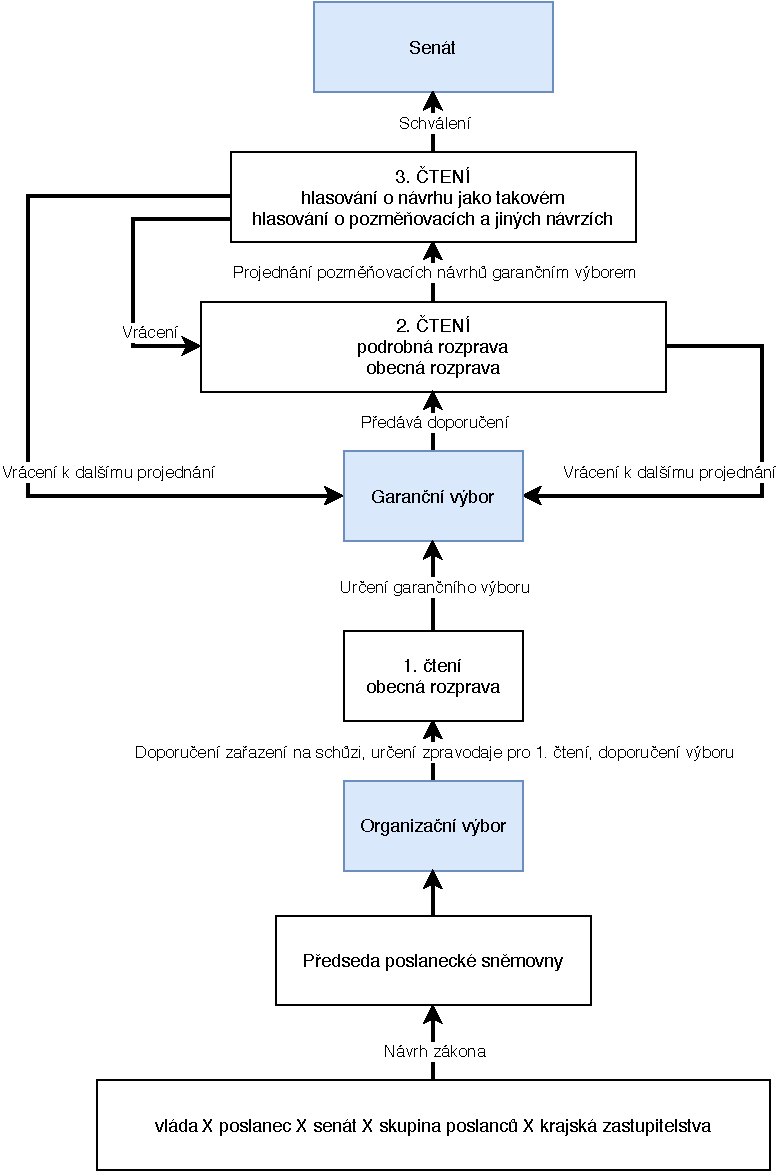
\includegraphics[width=0.9\textwidth]{obrazky-figures/legislativni_proces_my.pdf}
    \caption{Zjednodušený graf legislativního procesu v Poslanecké sněmovně}
    \label{fig:legislativni_proces}
\end{figure}
 
\subsection{Výbory poslanecké sněmovny}
\label{vybory}
\par Výbory poslanecké sněmovny jsou skupiny lidí zaměřené na určitý odborný problém, složené jak z členů vlády, tak opozice. Tyto skupiny se návrhem zákona zabývají v odborné rovině a následně na 2. čtení PS doporučí návrh přijmout, zamítnout, nebo navrhnou změny.\\
Jeden návrh může být přiřazen více výborům, každý z výborů má svého zpravodaje, ale jen jeden z nich je tzv. garanční - ručí za přidělený návrh. \\

\subsection{Jednání PS}
\par Jednání, na kterých jsou návrhy zákonů projednávány, se nazývají schůze Poslanecké sněmovny. Aby byla sněmovna usnášeníschopná, musí být přítomno alespoň třetinové kvórum, což odpovídá 67 poslancům. \cite{ustava-kvorum} \\
Průběh jednání z hlediska hlasování vypadá následovně:\\
\begin{itemize}
    \item Přihlášení účastníků
    \item Určení zapisovatelů a hlasování o jejich schválení
    \item Hlasování o jednotlivých bodech aktuální schůze \\
    - v případě, že vůbec dojde k jejich projednání
    \item Hlasování o pořadí projednávaných bodů
    \item Hlasování o konkrétních bodech na pořadu\\
    - může dojít ke zpochybnění hlasování a k jeho opakování \\
    \item V průběhu schůze může dojít také k některým dalším, méně zajímavým, hlasovnáním například o odložení projednávání nějakého aktuálního bodu na později, či vyhlášení přestávky.
    
\end{itemize}

\subsection{Kvórum}
Kvórum je minimální počet hlasů nutný pro přijetí návrhu hlasováním. Běžně je kvórum nadpoloviční většina přítomných poslanců, v některých případech se však může lišit. Například kvórum nadpoloviční většiny všech poslanců nutné pro přehlasování veta Senátu, či prezidenta, nebo kvórum 3/5 přítomných nutné pro přijetí ústavních zákonů \cite{zakon-kvorum}.

\subsection{Sněmovní tisky}
Sněmovní tisky jsou, zjednodušeně řečeno, dokumenty předkládané poslancům jako podklady pro jednotlivé body programu. 

\section{Existující řešení}
Na internetu lze v době psaní této práce nalézt více verzí českých i zahraničních volebních kalkulaček. Jelikož jsou volby obecně pro jednotlivé země silně specifické, zahraniční aplikace zde nebudu rozebírat. Z těch českých jsou nejzajímavější hlavně volebnikalkulacka.cz\footnote{volebnikalkulacka.cz: \url{https://volebnikalkulacka.cz/}} a ta na zpravodajském portálu iDnes.cz\footnote{Volební kalkulačka na idnes.cz: \url{https://volby.idnes.cz/volebni-kalkulacka-kraje.aspx}}. Za zmínku stojí také Postvolítko\footnote{Postvolítko: \url{https://www.fi.muni.cz/~xzahrad4/Hlasovatko/index.cgi?o=8}}, projekt studentů Masarykovy univerzity. 

\subsection{volebnikalkulacka.cz}
Princip této volební kalkulačky  je jednoduchý. Autor, či autoři, vytvoří soubor otázek, který by podle jejich názoru mohl uživatele zajímat. Tyto otázky jsou následně rozeslány všem zúčastněným politickým stranám, či kandidátům. Na základě matematických modelů jsou poté odpovědi zpracovány a vybrány nejlepší otázky. Tyto jsou nakonec prezentovány v samotné kalkulačce (obr. \ref{fig:volebnikalkulacka-otazka}), kde na ně odpovídá uživatel. Po ukončení dotazníku je uživateli představena jeho procentuální shoda v odpovědích s jednotlivými stranami či kandidáty (obr. \ref{fig:volebnikalkulacka-vysledky}) \cite{volebnikalkulacka-info}.
\par Výhoda tohoto systému je v jeho jednoduchosti a přehlednosti. Otázky bývají jednoznačné, srozumitelné a týkají se aktuálních témat, takže běžný uživatel nemusí mít nic než obecný přehled o hlavním dění v České republice a ve svém kraji. 
\par Za jeho nevýhodu by se dala považovat závislost na pravdivých odpovědích a nepopulistickém přístupu. Může se totiž stát, že kandidát vyplní dotazník podle toho co zrovna v tu chvíli jeho potenciální voliči požadují a následně ve skutečných hlasováních v Poslanecké sněmovně hlasovat jinak.
\\

\begin{figure}
    \centering
    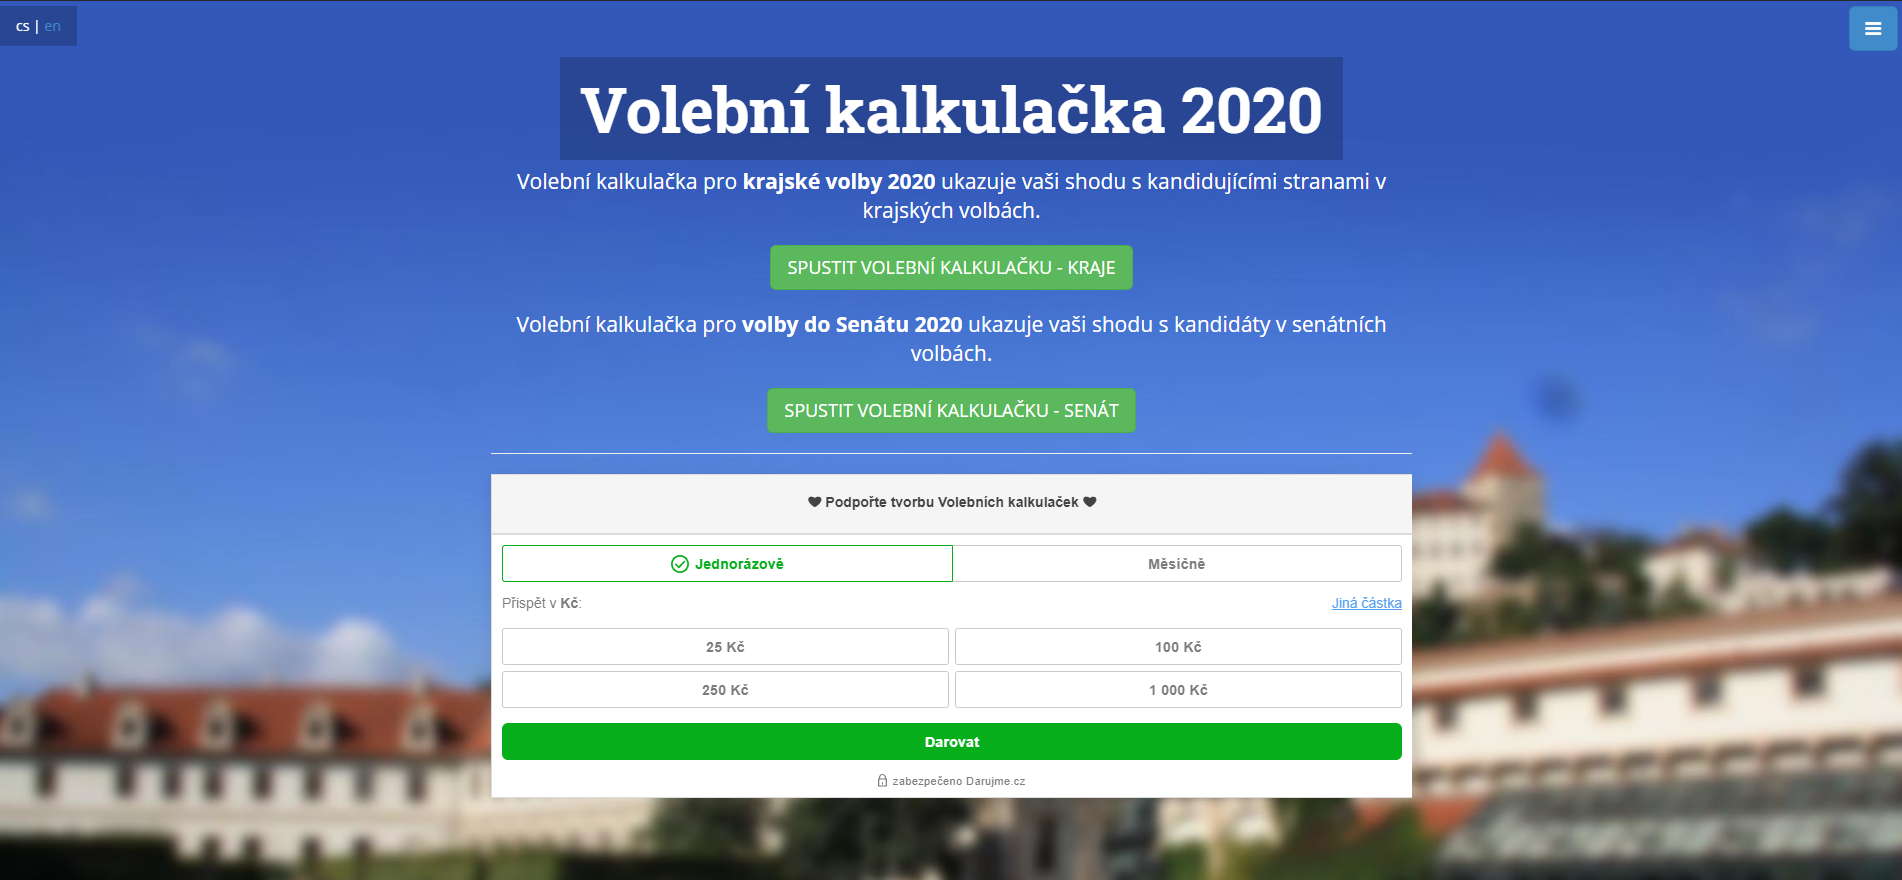
\includegraphics[width=1\textwidth]{obrazky-figures/volebnikalkulackacz-uvod.png}
    \caption{Úvodní stránka aplikace volebnikalkulacka.cz}
    \label{fig:volebnikalkulacka-uvod}
\end{figure}

\begin{figure}
    \centering
    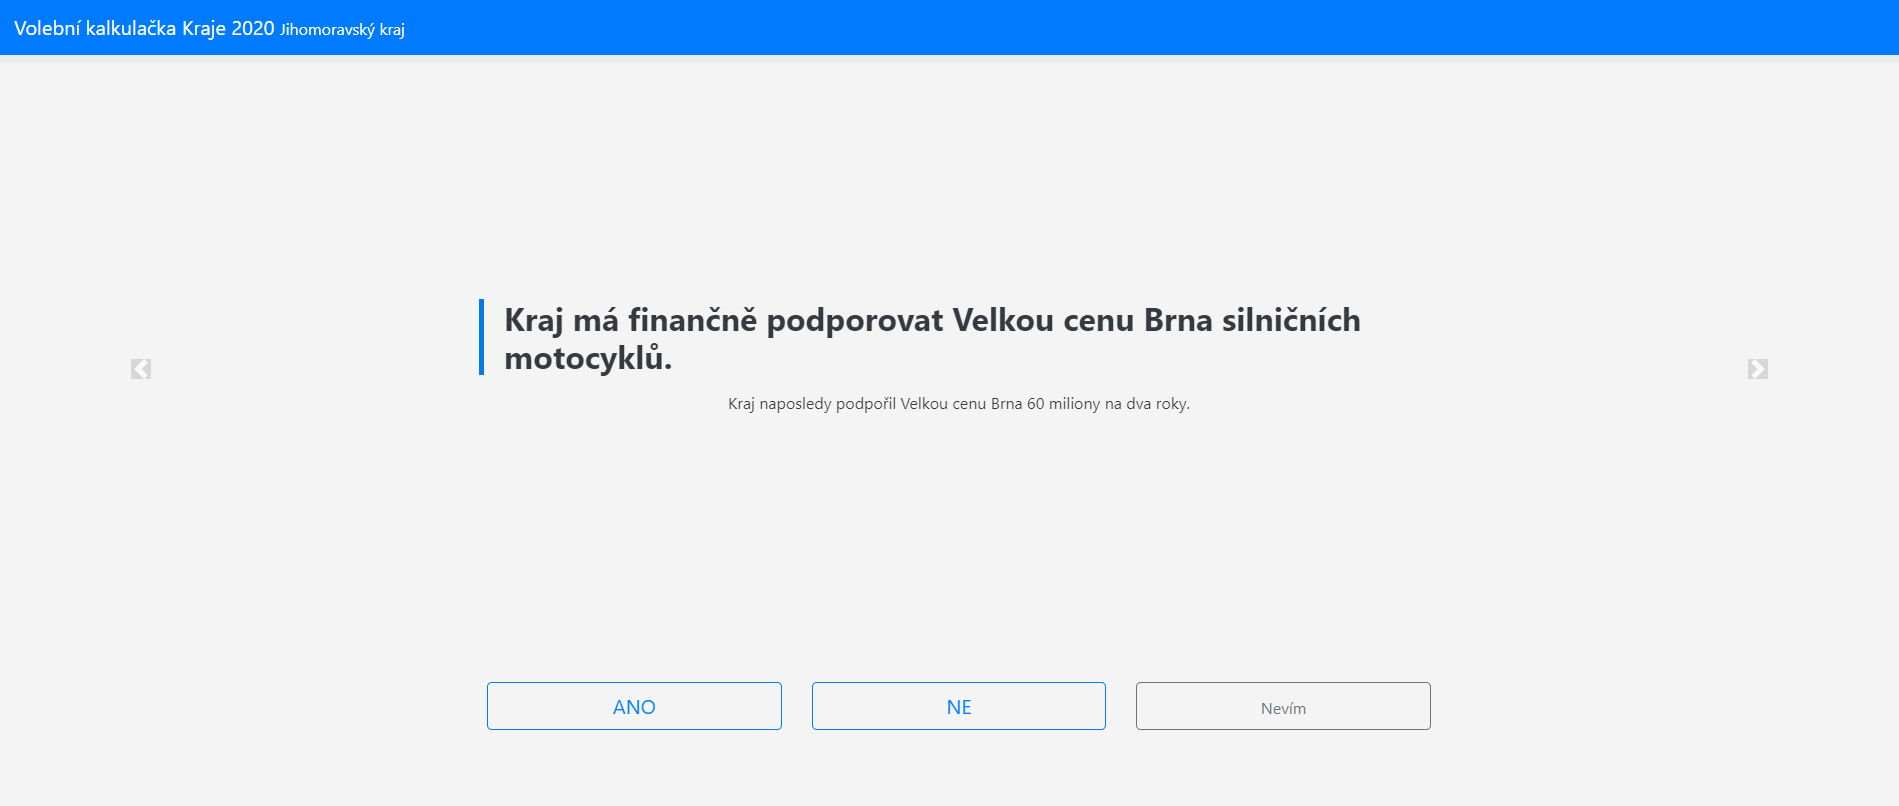
\includegraphics[width=1\textwidth]{obrazky-figures/volebnikalkulacka-otazka.png}
    \caption{Příklad otázky v aplikaci volebnikalkulacka.cz}
    \label{fig:volebnikalkulacka-otazka}
\end{figure}

\begin{figure}
    \centering
    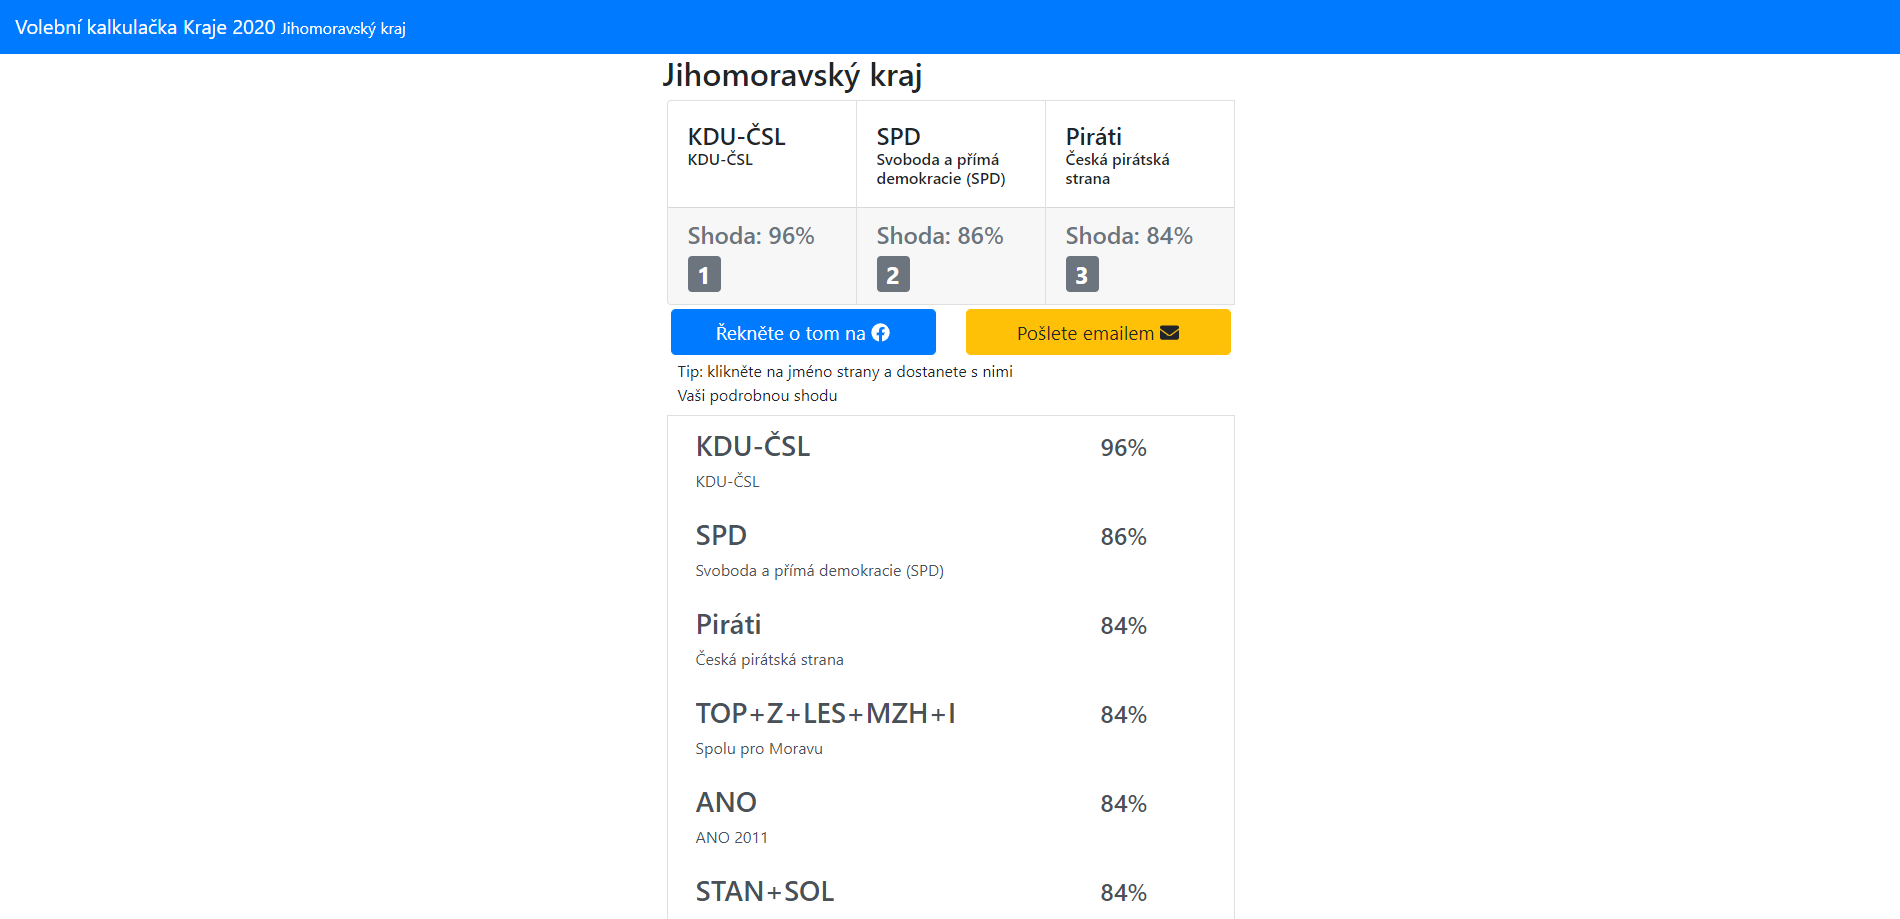
\includegraphics[width=1\textwidth]{obrazky-figures/volebnikalkulacka-vysledky.png}
    \caption{Příklad prezentace výsledků uživateli v aplikaci volebnikalkulacka.cz}
    \label{fig:volebnikalkulacka-vysledky}
\end{figure}




\subsection{iDnes.cz}
Princip této aplikace je totožný jako u volebnikalkulacka.cz. Liší se pouze některé otázky a grafický vzhled, který je zde přizpůsoben celkovému stylu zpravodajského webu idnes.cz,\footnote{idnes.cz: \url{https://www.idnes.cz/}} viz obrázek \ref{fig:idnes-uvod}. Dokonce mají obě aplikace i stejného autora, kterým je sdružení \mbox{kohovolit.eu}.\footnote{kohovolit.eu: \url{http://kohovolit.eu/}}

\begin{figure}
    \centering
    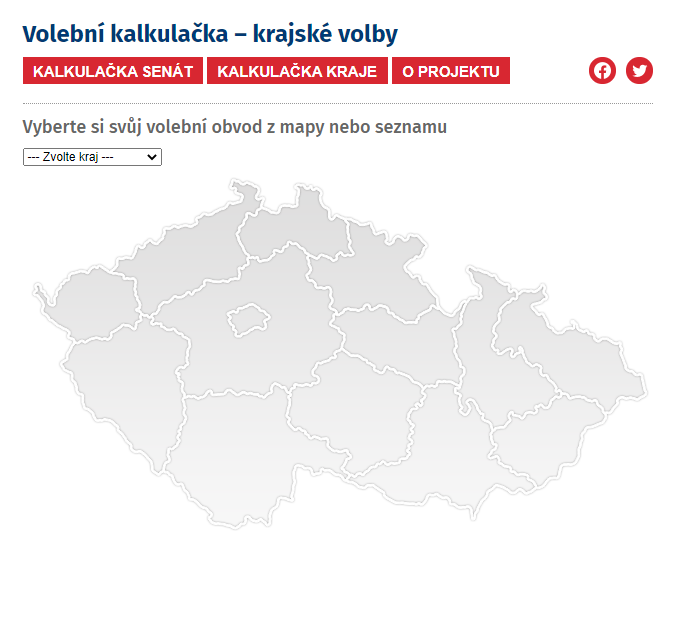
\includegraphics[width=0.7\textwidth]{obrazky-figures/idnes-uvod.png}
    \caption{Úvodní strana volební kalkulačky na webu Idnes.cz}
    \label{fig:idnes-uvod}
\end{figure}

\subsection{Postvolítko}
Přestože nejde o volební kalkulačku, je tato studentská aplikace velmi zajímavý nástroj pro zkoumání dat z Poslanecké sněmovny. Ta jsou zde přehledně a srozumitelně rozřazena do 3 různých přehledů - hlasování, poslanci a strany, jak můžeme vidět na obrázku \ref{fig:postvolitko-uvod}.

\begin{figure}
    \centering
    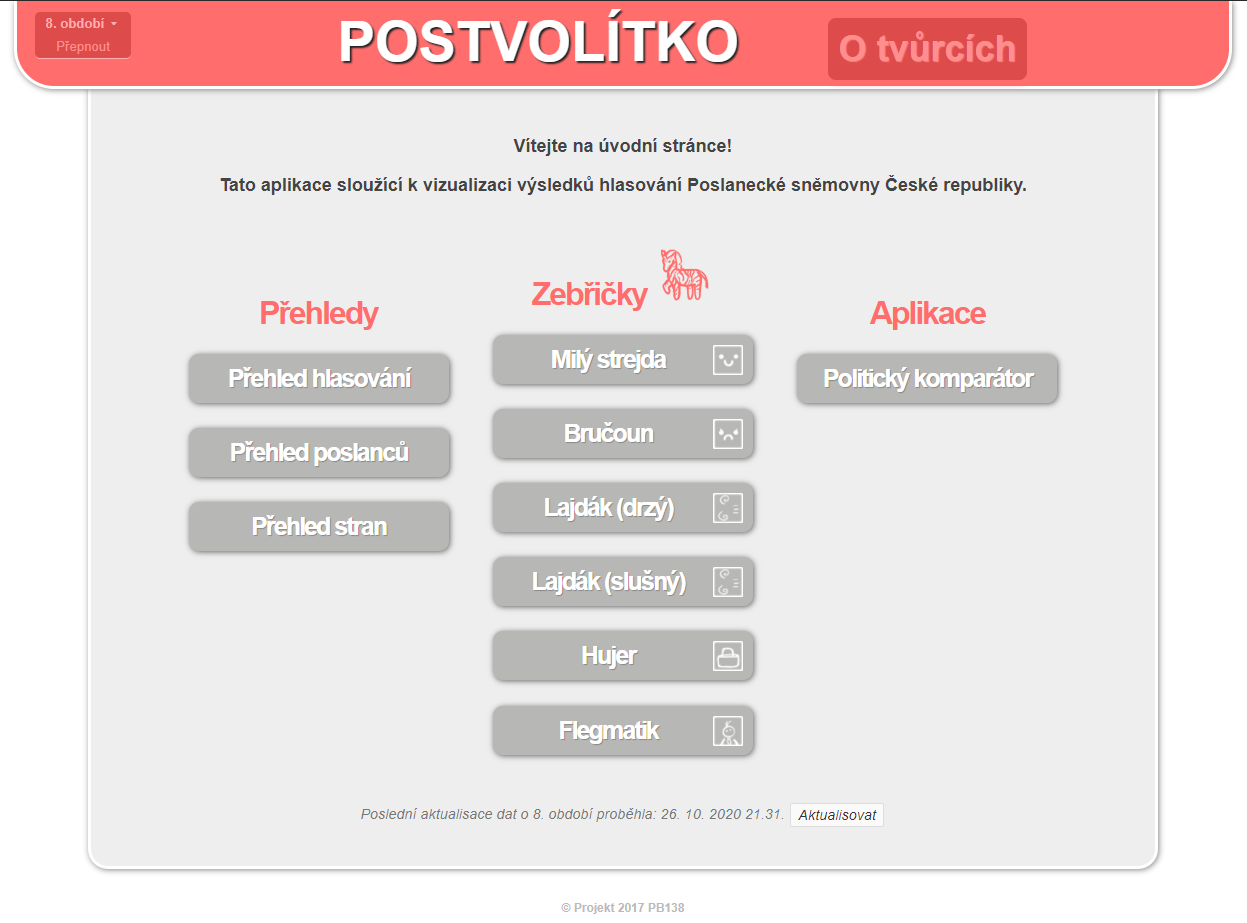
\includegraphics[width=0.7\textwidth]{obrazky-figures/postvolitko-uvod.png}
    \caption{Úvodní strana webové aplikace Postvolítko}
    \label{fig:postvolitko-uvod}
\end{figure}


\par Přehled hlasování nabízí výčet všech poslaneckých schůzí ve zvoleném volebním období. Tyto schůze jsou dále doplněny o přehled jednacích bodů schůze a k nim náležejících hlasování, obr. \ref{fig:postvolitko-hlasovani}. \\
U jednotlivých hlasování lze dále otevřít detail s konkrétními jmény poslanců a jejich volbou.

\begin{figure}
    \centering
    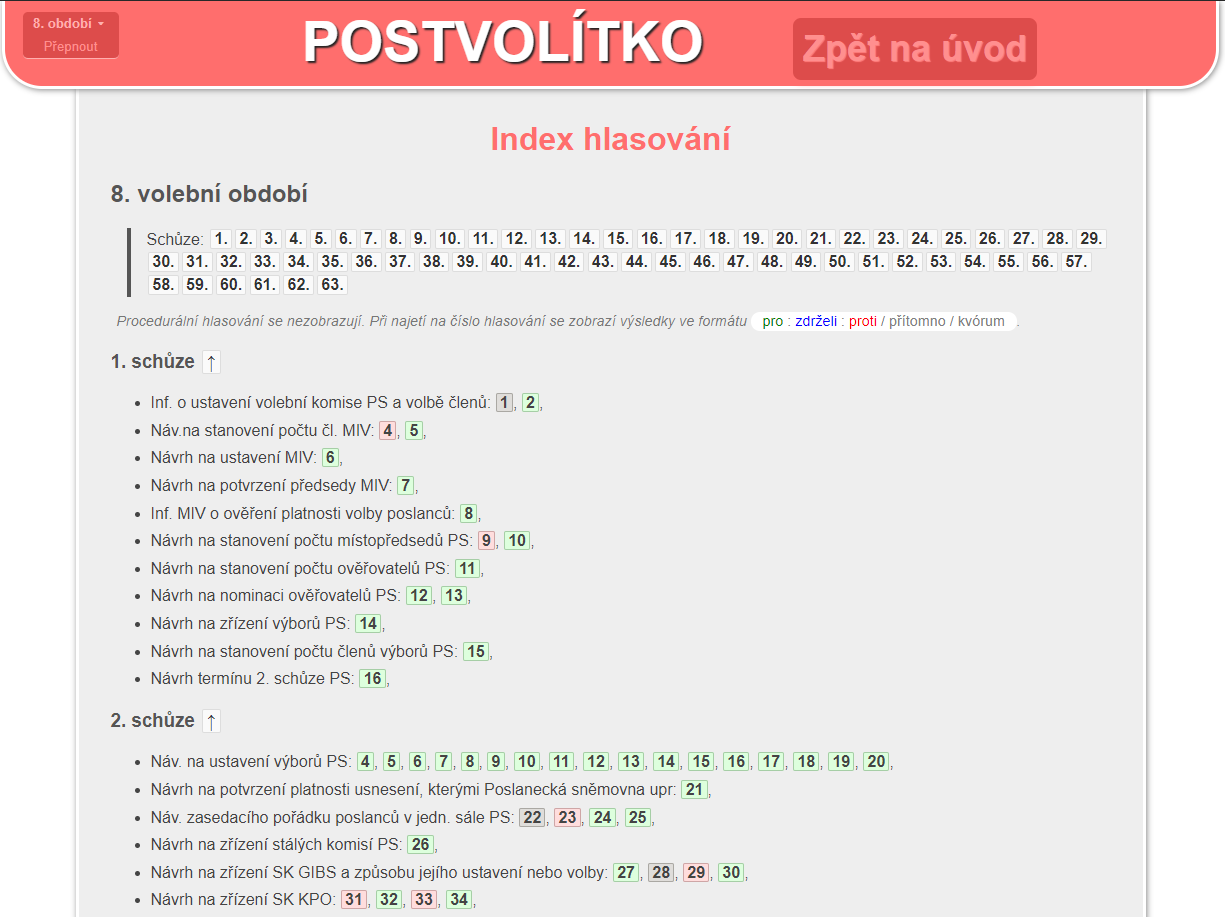
\includegraphics[width=0.7\textwidth]{obrazky-figures/postvolitko-hlasovani.png}
    \caption{Přehled schůzí a hlasování PS v aplikaci Postvolítko}
    \label{fig:postvolitko-hlasovani}
\end{figure}

\par Přehled poslanců nabízí seznam všech aktivních poslanců ve zvoleném volebním období. Pod jménem poslance se dále lze dostat na detail jeho osoby, kde nalezneme kromě jeho veřejně dostupných osobních údajů také statistiky jeho hlasování a absencí.


\par V přehledu stran nalezneme seznam všech aktuálně zúčastněnch stran v poslanecké sněmovně. Přes jednotlivé strany se dá opět dostat na jejich detail. Zde je opět seznam poslanců, pouze omezen na členy konkrétní strany.

\par Dále zde nalezneme žebříčky podle různých statistik, například podle počtu hlasování pro, počtu neomluvených hodin, či nejnižší absence. 
\par Poslední funkcí Postvolítka je porovnávání dvou vybraných poslanců a zobrazení jejich procentuální shody, vycházející ze stejných voleb u jednotlivých hlasování.


\section{Výchozí data}
Data, ze kterých tato práce čerpá, se nachází na oficiálním webu Poslanecké sněmovny Parlamentu České republiky\footnote{Oficiální web Poslanecké sněmovny: \url{https://www.psp.cz/sqw/hp.sqw}}. Konkrétně se jedná o data agend Poslanecké sněmovny\footnote{Data agend Poslanecké sněmovny: \url{https://www.psp.cz/sqw/hp.sqw?k=1300}}, poskytovaná veřejnosti zdarma pod podmínkou uvedení zdroje a data zpracování\cite{pspData}.
\par Zde dostupné záznamy popisují všechny schůze Poslanecké sněmovny až do roku 1993. Ty jsou dále děleny na popis samotné schůze a jejího stavu, jednotlivé body pořadu, jejich popis, stav a výsledek. Kromě samotných schůzí jsou k dispozici také záznamy o všech poslancích v tomto volebním období - fotky, pracovní emaily a telefony, ostatní funkce které vykonávají, či jejich hlasování a absence.
\par Data jsou strukturována v tabulkách, mezi nimiž jsou vzájemné vazby. Na obrázku \ref{fig:psp-tabulka-priklad} je struktura jedné z databázových tabulek. Ty nejpodstatnější vazby mezi tabulkami pro tuto práci jsou naznačeny na obrázku \ref{fig:psp-data-diagram}.
\par Jednou denně jsou všechna data aktualizována a doplněna o nové záznamy. Tato aktualizace probíhá v noci.



\begin{figure}
    \centering
    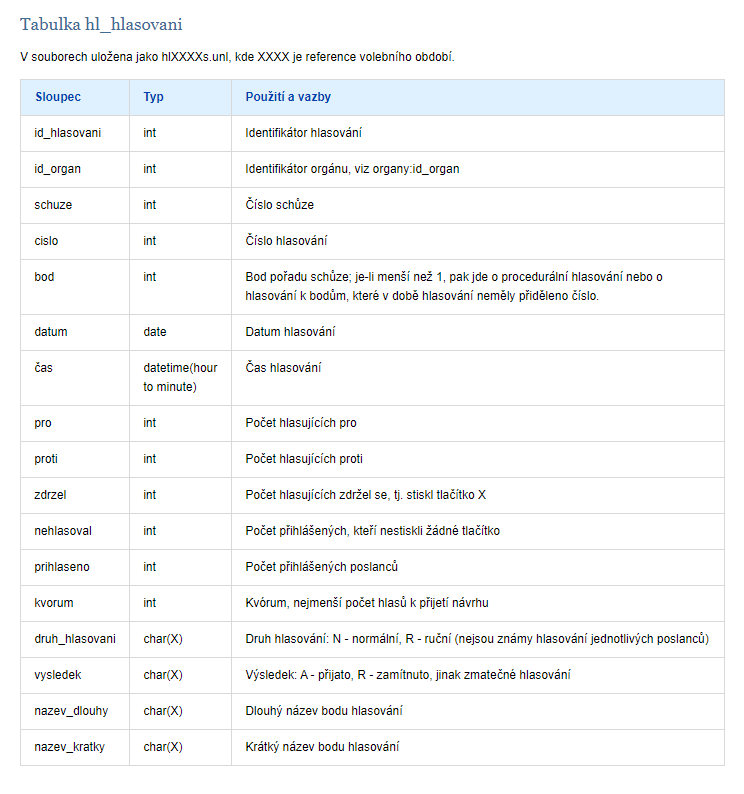
\includegraphics[width=0.8\textwidth]{obrazky-figures/psp-tabulka-priklad.png}
    \caption{Popis struktury jedné z datových tabulek Poslanecké sněmovny\cite{pspData}}
    \label{fig:psp-tabulka-priklad}
\end{figure}

\begin{figure}
    \centering
    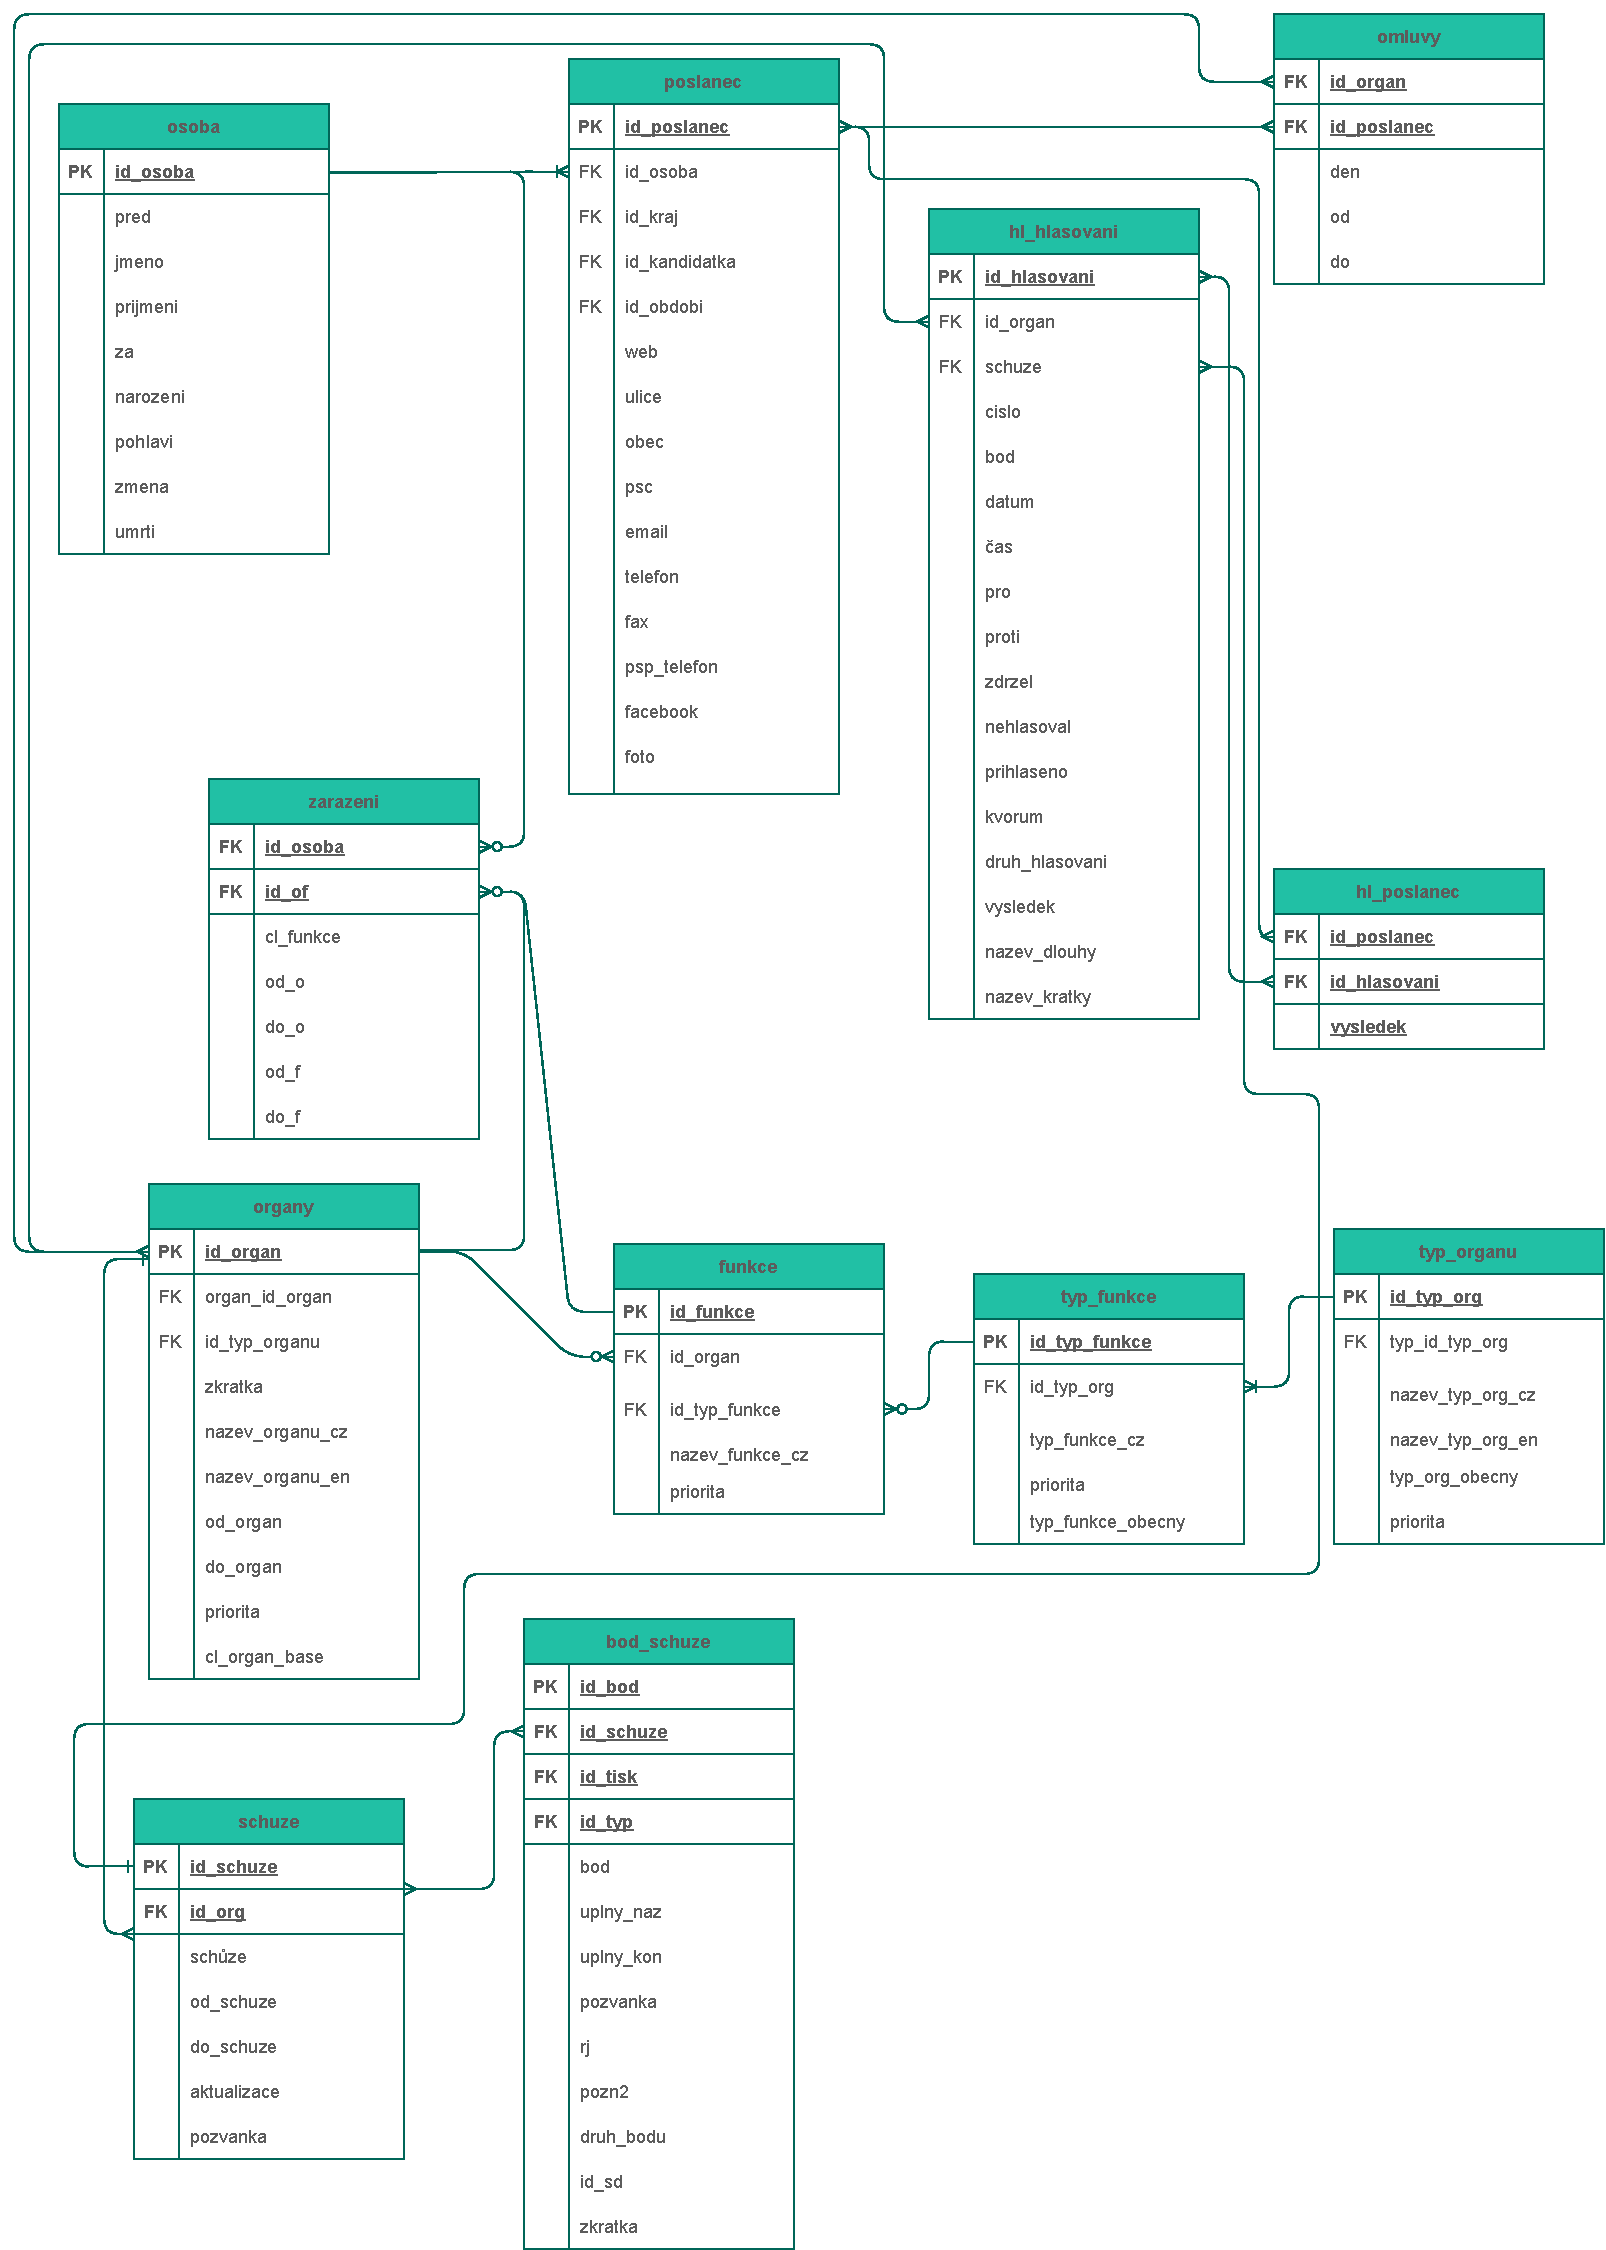
\includegraphics[width=1\textwidth]{obrazky-figures/data_diagramy.pdf}
    \caption{Diagram znázorňující vztahy některých datových tabulek}
    \label{fig:psp-data-diagram}
\end{figure}




%%%%%%%%%%%%%%%%%%%%%%%%%% TECHNOLOGIE  %%%%%%%%%%%%%%%%%%%%%%%%%%%%%%%
\chapter{Použité technologie}
\label{chap:technologie}
V této kapitole jsou stručně popsány použité technologie. Jedná se o webovou stránku, proto jsou na úvod představeny základní techniky k vytvoření statického webu. Po nich následuje představení technologií zajišťujících dynamičnost. Zde patří python a jeho framework Django. Pro nasazení na produkčním serveru a mezipaměť (anglicky \texttt{cache}) jsou využity technologie Docker\footnote{Docker: \url{https://www.docker.com/}} a Redis\footnote{Redis: \url{https://redis.io/}}, které propojuje s vnějším světem technologie Traefik\footnote{Traefik: \url{https://doc.traefik.io/traefik/}}.
\par Kapitola je zakončena popisem použitého databázového systému PostgreSQL.


\section{HTML, CSS}
HTML je zkratka pro \texttt{hyper text markup language}. Jak už název napovídá, tento jazyk není programovací, nýbrž strukturovací (značkovací). To znamená, že pomocí něj dokážeme vytvořit strukturu a význam částí dokumentu, který následně dokáží správně zobrazit a interpretovat webové prohlížeče. Často se přirovnává ke kostře lidského těla.  \cite{HTML}

\par CSS je zkratkou pro \texttt{cascading style sheets} a definuje jak budou HTML elementy zobrazeny. V překladu název znamená "kaskádové styly", kdy kaskádě odpovídá vrstvení jednotlivých stylů na sebe, ovšem vždy platí ten poslední, případně ten nejspecifičtější. Při použití předchozího přirovnání by CSS bylo jako maso a kůže. \cite{CSS} 


\section{Bootstrap}
Bootstrap\footnote{Bootstrap: \url{https://getbootstrap.com/}} je aktuálně nejpoužívanější CSS framework pro vývoj responsivních a tzv. \texttt{mobile-first} stránek. \cite{BOOTSTRAP} Poskytuje předpřipravené HTML a CSS komponenty, pomocí kterých se dá rychle a jednoduše vytvořit design webu. Klíčovým aspektem je využívání tříd, kterými je vývojář schopen jednoduše přiřadit HTML elementům styly, které bootstrap již v základu poskytuje, aniž by při tom musel neustále přecházet mezi HTML šablonou a CSS dokumentem. Jednou z nejvyužívanějších funkcí bootstrapu je možnost virtuálního rozdělení obsahu elementu na 12 stejných sloupců, se kterými lze pak jednoduše pracovat pomocí přidávání tříd na elementy obsahu. Velkou výhodou je také jednoduchá práce s responsivitou, opět pomocí různých tříd.
\par  Obecně existují dva způsoby myšlení při vytváření webové stránky. První je navrhnout nejprve verzi pro stolní počítače, respespektive celkově velké obrazovky a pak ji postupně obírat o funkcionalitu, aby byla použitelná i na telefonu. Tento způsob byl přijatelný dříve, kdy mobilní telefony sloužily primárně k telefonování a počet návštěvníků webu z nich nebyl nijak závratný. Se zvyšujícím se využitím mobilních telefonů pro prohlížení internetu, kdy v dnešní době více než polovina lidí tzv. "surfuje"\ na telefonu \cite{WEB-DEVICE-USAGE}, je však již považován za nedostatečný.
\par Tím druhým je právě \texttt{mobile first}, kdy se nejprve navrhne design pro mobilní telefony a až s přibývajícím místem na obrazovce se doplňují i pokročilejší designové prvky a funkce. Tento způsob je v současné době obecně využívanější, jelikož je pro vývojáře ve většině případů mnohem komfortnější a zaměřuje se primárně na jednoduchost a ovladatelnost právě na malých obrazovkách, kde to mnohdy může být pro uživatele problém.

\section{Sass}
Sass\footnote{Sass: \url{https://sass-lang.com/}} je jeden z několika běžně používaných CSS preprocesorů.\footnote{CSS preprocesory: \url{https://raygun.com/blog/css-preprocessors-examples/}} Ve své podstatě je CSS preprocesor nástroj, respektive jazyk, který zjednodušuje, zpřehledňuje a zrychluje aplikaci CSS webových stránek. Snaží se zvýšit efektivitu psaní kódu pomocí minimalizace nutnosti kopírovat velké bloky již jednou napsaného kódu, což je konkrétně u CSS běžná věc. Přidává například možnost použití proměnných, zanořování selektorů, využívání mixinů. 
\par Prohlížeče nicméně stále ještě pracují pouze s čistým CSS, proto se do něj jazyk preprocesorů musí překládat před tím, než ho server odešle uživateli. 


\section{JavaScript}
JavaScript\footnote{JavaScript: \url{https://developer.mozilla.org/en-US/docs/Web/JavaScript}} je scriptovací jazyk umožňující dynamicky měnit obsah stránky bez nutnosti stránku znovu načíst. Kromě toho umí také spoustu dalších věcí, kupříkladu ovládat multimédia a animovat jednotlivé elementy. Naprostá většina moderních prohlížečů má jeho podporu již vestavěnou, mezi výjimky patří například textový prohlížeč Lynx\footnote{Lynx: \url{https://lynx.browser.org/}}. Podle dostupných statistik \cite{JAVASCRIPT-USAGE} je dnes JavaScript využíván na 95\% webových stránek.

\section{jQuery}
jQuery\footnote{jQuery: \url{https://jquery.com/}} je malá knihovna určená ke zjednodušení práce s JavaScriptem. Hlavní snahou je zmenšení množství napsaného kódu, nutného k vytvoření požadované funkcionality, spolu se zjednodušením používání některých JavaScriptových prvků, kupříkladu AJAX\footnote{AJAX: Asynchronní JavaScript a XML} volání. \cite{JQUERY} Další z výhod jQuery je obrovské množství dostupných pluginů, díky kterému je často možné jednoduše odstranit i komplikované problémy pomocí již hotového řešení.\footnote{jQuery pluginy: \url{https://plugins.jquery.com/chosen/}}  
\par jQuery je v současné době nejspíše nejpopulárnější JavaScriptový framework, využívaný na více než 19 milionech webových stránek \cite{JQUERY-USAGE}. Najdeme ho obsažen také v populárním systému správy obsahu Wordpress\footnote{Wordpress: \url{https://wordpress.org/}}, nicméně postupně se objevuje snaha od jeho použití upouštět kvůli zbytečnému zvyšování velikosti stránky.

\section{Python}
"Python\footnote{Python: \url{https://www.python.org/}} je interpretovaný, objektově orientovaný, vysokoúrovňový programovací jazyk s dynamickou sémantikou." \cite{PYTHON} \\
Kromě toho je v současné době asi nejrychleji rostoucím a nejoblíbenějším programovacím jazykem napříč celou škálou oborů, díky své jednoduchosti a intuitivnosti. Využívá se ve všech možných aplikacích, od základní automatizace opakujících se činností, například zpracování excelu, nebo zpracování dat z webových stránek, přes matematické operace, analýzu a vizualizaci dat, až po vytváření umělé inteligence. Mimo to ho lze využít také k vytváření aplikací, mobilních, desktopových i webových. Právě kvůli možnosti vytvoření webové aplikace, která bude zároveň mít možnost zpracovávat a analyzovat data bez nutnosti přidávání dalších nástrojů, byl jazyk python zvolen pro serverovou část této práce.

\section{Django}
Django\footnote{Django: \url{https://www.djangoproject.com/}} je volně dostupný, open-source framework pro webové aplikace napsané v jazyce Python. Jeho smyslem je ulehčit a urychlit vytváření webových aplikací. Za tímto účelem poskytuje již předpřipravenou strukturu, zajišťující například zabezpečení, práci s databází, šablonování, autentizaci a další. Django vychází z návrhového vzoru MVC, což je jeden z nejpopulárnějších návrhových vzorů využívaných pro webové stránky, kde \texttt{Controller} je nahrazen šablonami (anglicky "Template"), tedy \texttt{MVT}. Kromě toho Django obsahuje množství volně dostupných zásuvných modulů (\texttt{pluginů}) rozšiřujících jeho funkcionalitu. Nechybí také přehledná a rozsáhlá dokumentace a široká uživatelská základna nabízející pomoc při řešení problémů.

\subsubsection{MVT}
MVT, čili \texttt{model-view-template} je návrhový vzor rozdělující aplikaci na 3 základní části. Model je databázová část, starající se o to jak jsou data uchovávána, o jejich ukládání a čtení. View obsahuje logiku a komunikuje s Modelem. Template je HTML šablona, které View předá data a kterou django nakonec zobrazí (vyrenderuje) uživateli. Diagram fungování MVT je znázorněn na obrázku \ref{fig:MVT}

\begin{figure}
    \centering
    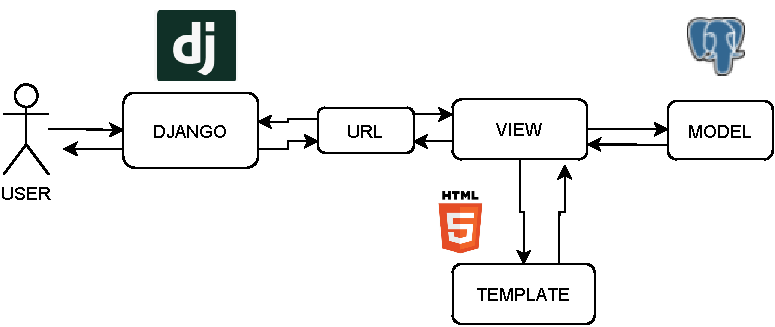
\includegraphics[width=0.8\textwidth]{obrazky-figures/MVT.pdf}
    \caption{Fungování návrhového vzoru MVT}
    \label{fig:MVT}
\end{figure}

\section{Cookiecutter}
Cookiecutter-Django\footnote{Cookiecutter: \url{https://github.com/pydanny/cookiecutter-django}} je generátor základní kostry Django webové aplikace. Uživatel si při spuštění generátoru postupně vybírá jaké technologie chce ve svém projektu použít a aplikace mu podle toho sestaví plně funkční základní moduly a soubory. Díky tomu si projekt udržuje určitý vhodný systém a uspořádání už od počátku.

\section{Docker}
Docker je, zjednodušeně řečeno, virtualizační nástroj umožňující umístit aplikaci spolu se všemi jejími potřebami na server nezávisle na jeho druhu a nainstalovaných aplikacích. Docker kontejner poskytuje základní, předpřipravené prostředí, ve kterém aplikace následně běží, podobně jako běžné virtualizované systémy. Jeho výhodou však je, že na rozdíl od nich není tak náročný, je menší a jednodušeji spravovatelný.  

\par Každá služba má svůj vlastní Docker kontejner - jeden kontejner zvlášť pro každou ze služeb Redis, PostgreSQL, Django a Traefik. Tyto mezi sebou můžou komunikovat díky propojení vlastní lokální sítí. 

\par 
Aby nebylo potřeba ručně při každém zapnutí aplikace konfigurovat každý z kontejnerů zvlášť, existuje \texttt{docker-compose}. Správce aplikace sepíše všechno nastavení do souboru zvaného \texttt{Dockerfile} a docker-compose se po spuštění postará o zbytek.

\section{Redis}
Redis je NoSQL\footnote{NoSQL: \url{https://aws.amazon.com/nosql/}} databáze. Běžné SQL databáze využívají k ukládání dat tabulky, které jsou dále členěny na sloupce a řádky, kdy sloupce mají pevně daný typ dat které mohou obsahovat. Redis využívá dvojice klíč:hodnota, kde hodnota může nabývat jeden z několika typů. Je schopen celý pracovat uvnitř paměti, což z něj činí velmi rychlý a efektivní nástroj vhodný pro použití jako cache, kdy díky němu můžeme místo zatěžování serveru opakovanými náročnými operacemi pouze vyčíst již jednou získané výsledky z mezipaměti s velmi nízkými náklady. V současné době je tímto způsobem využíván například například na Twitteru, StackOverflow či Pinterestu.

\section{Traefik}
Traefik je open source proxy. Jeho úlohou je v našem případě mapování vnějších portů na aplikaci. Tzn. pokud někdo přistoupí na adresu serveru na port 80, Traefik tento přístup přepošle(přeloží) na port v django docker kontejneru. Konkrétní port závisí na nastavení v Dockerfile.


\section{PostgreSQL}
PostgreSQL\footnote{PostgreSQL: \url{https://www.postgresql.org/}} je výkonný objektově-relační, open-source, databázový systém využívající a zároveň rozšiřující jazyk SQL. Jeho vznik se datuje až do roku 1986 a za dobu své existence si získalo pověst spolehlivého, robustního a jednoduše rozšiřitelného řešení databáze. \cite{PostgreSQL}
\par Při volbě databázového systému byl původní kandidát MySQL, jelikož s ním často pracuji a všechno potřebné jsem tak měl již připravené. Nicméně podle některých názorů \cite{WHY-POSTGRES1}\cite{WHY-POSTGRES2} je obecně lepší využívat databázový systém PostgreSQL, jelikož je na něj Django lépe připravené a používají ho i sami vývojáři, takže bude lépe dokumentován.

\section{Další technologie}
Za zmínku stojí také \texttt{npm}, což je nejpoužívanější správce javascriptových balíčků. 



%%%%%%%%%%%%%%%%%%%%%%%%%% Návrh %%%%%%%%%%%%%%%%%%%%%%%%%%%%%%%
\chapter{Návrh aplikace}
\label{chap:navrh}
U webových aplikací obecně platí, že rozhodnutí uživatele o využití či opuštění stránky z velké části závisí na designu, použitelnosti ale hlavně prvním dojmu. Proto je třeba, aby kromě kvalitní funkcionality měla aplikace také moderní a promyšlený vzhled. \\
Nejprve je třeba vytyčit cílovou skupinu. Díky tomu zjistíme, na jaké části systému je třeba se zaměřit a případně jakým způsobem je nejlépe zpracovat pro co největší uživatelský komfort. Dalším krokem je analýza případů užití, pomocí které zjistíme, jaké funkce budou uživatelé potřebovat a používat. Následuje návrh databáze, vycházející z dat, se kterými chceme pracovat a z jejich vztahů. Kapitola vrcholí samotným grafickým návrhem, zpracovávajícím všechny předchozí kroky do jednoho úhledného a intuitivního uživatelského rozhraní.


\section{Cílová skupina}
Cílová skupina kalkulačky budou obecně všichni lidé s volebním právem, tedy občané České republiky starší 18-ti let.\cite{ustava-volebni_pravo} Podle statistiky zveřejněné na webu statistikaamy.cz\footnote{statistikaamy.cz: \url{www.statistikaamy.cz}}, který spravuje Český statistický úřad\footnote{Český statistický úřad: \url{https://www.czso.cz/csu/czso/domov}}, používalo v roce 2016 internet 32,5\% z lidí starších 65 let\cite{statistikaamy}. Bude tedy třeba zvýšit důraz na jednoduchost, přehlednost a intuitivnost, které jsou zejména pro starší lidi kritické.
\par Dále lze tuto skupinu rozdělit na dvě menší části. Tou první jsou lidé, kteří využíjí naplno všech funkcí webu, včetně registrace a uložení výsledků na svůj profil, hodnocení poslanců a komentářů. Zde budou spadat zejména mladší uživatelé. Pro ty bude důležité, aby registrace byla jednoduchá a rychlá a zároveň jim web umožňoval spravovat svůj profil a své uložené výsledky. 
\par Zbylá část bude tvořena lidmi, které bude zajímat pouze jejich výsledek a hned po jeho zjištění web opustí. V tomto případě je nutné co nejvíce zjednodušit přístup k hlavní funkční části webu. \todo{Upravit podle reality}


\section{Případy užití}
Po příchodu na web uvidí každý uživatel domovskou stránku, poskytující základní přehled o smyslu a cíli aplikace. Na výběr zde má celkem tři akční oblasti. Kromě horního menu a patičky, které jsou přístupny na každé stránce aplikace, také velké akční tlačítko sloužící pro přechod do kalkulačky. Použití kalkulačky je pro všechny uživatele stejné, liší se až konec, kdy registrovaný a přihlášený uživatel může využít možnosti uložit si právě získané výsledky ke svému profilu. Každý uživatel může také své výsledky sdílet na sociálních sítích. 
\par Horní menu odkazuje na jednotlivé části aplikace, na přehledy poslanců, hlasování a stran, které může použít každý uživatel. Je zde také tlačítko pro přihlášení, případně odkaz na uživatelský účet, pokud již uživatel přihlášený je. Pokud není, je mu přes něj umožněno se buď přihlásit, nebo přejít dalším odkazem na registrační formulář. Z přehledu poslanců se dá následně přejít na detail jednotlivých poslanců. Zde může registrovaný uživatel ohodnotit konkrétního poslance pomocí hvězdiček, či přidat komentář. Tyto dvě funkce byly omezeny pouze pro přihlášené uživatele z důvodu možného falšování hodnocení, či urážlivých komentářů. 
\par Přihlášeným uživatelům se přechodem do jejich účtu umožní upravovat svůj profil - přidat či upravit profilovou fotku, změnit heslo, spravovat svoje uložené výsledky.
\par V patičce pak má každý uživatel přístup k informacím o webu a ke stránce s kontakty.

\par
Případy užití znázorňuje diagram případů užití na obrázku \ref{fig:diagram_uc}

\begin{figure}
    \centering
    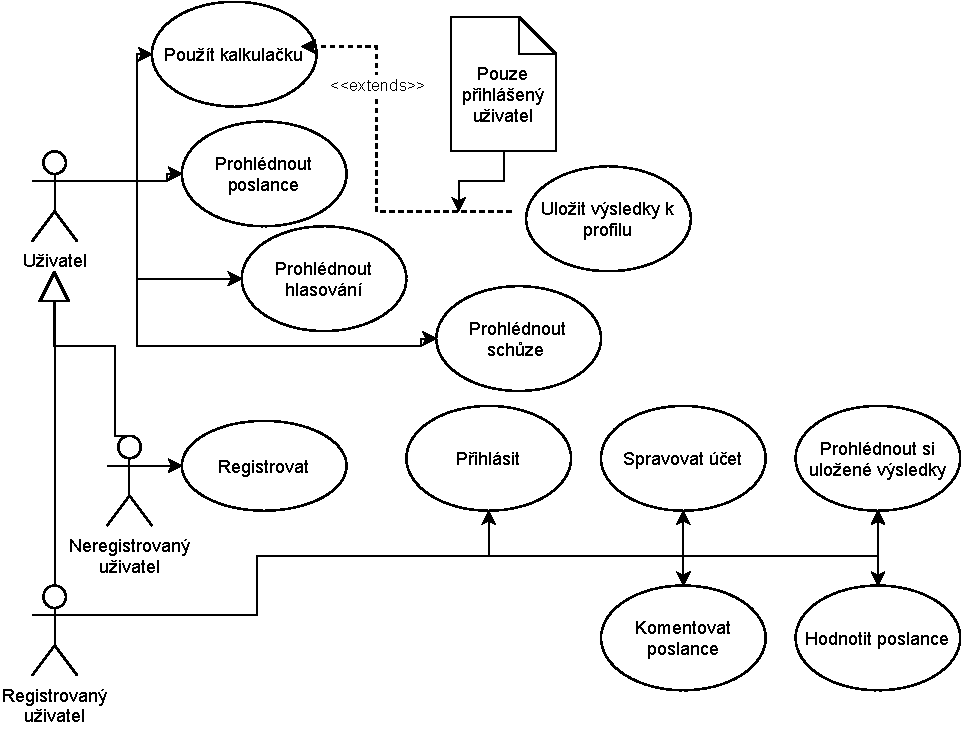
\includegraphics[width=0.8\textwidth]{obrazky-figures/UC.pdf}
    \caption{Diagram případů užití pro volební kalkulačku}
    \label{fig:diagram_uc}
\end{figure}



\section{Návrh databáze}
Největší část databáze tvoří tabulky převzaté z výchozích dat. Zde prakticky nedošlo k žádným úpravám vůči jejich popisu na webu Poslanecké sněmovny\footnote{Data PSP: \url{https://www.psp.cz/sqw/hp.sqw?k=1301}}. Pro uložení ohodnocení jednotlivých podstatných hlasování bylo nutno přidat tabulku \texttt{hl\_hlasovani\_rating}, uchovávající ohodnocení ke každému hlasování. Mimo to Django také potřebuje tabulky k uchovávání informací o registrovaných uživatelích a jejich oprávněních, či databázových migracích, což jsou zjednodušeně řečeno záznamy o změnách databázové struktury. Dále byly přidány také tabulky pro ukládání komentářů a hvězdičkových hodnocení jednotlivých poslanců. Všechny tabulky a jejich vzájemné vztahy jsou znázorněny v příloze \todo{cislo prilohy}.

\par Tabulek je příliš velké množství na popis, nicméně za zmínku stojí hlavně tabulky \texttt{hl\_hlasovani} uchovávající informace o jednotlivých hlasováních, \texttt{hl\_poslanec}, uchovávající všechna data o hlasování jednotlivých poslanců pro každé z existujících hlasování v předchozí tabulce, \texttt{hist} která je využita pro získání informací pro zjištění důležitých hlasování, \texttt{organy} uchovávající informace o orgánech, což můžou být strany, skupiny poslanců, volební období, výbory, a podobně. Dále také tabulka \texttt{zarazeni}, kde nalezneme  informace o zařazení jednotlivych poslanců v orgánech, tabulka \texttt{osoby}, která uchovává informace o jednotlivých osobách a na kterou se odkazuje tabulka poslanec.

\section{Drátový model}
\label{section:wireframe}
Drátový, nebo-li takzvaně \texttt{wireframe} model, slouží ke zjednodušené vizualizaci umístění jednotlivých prvků webu v prostoru. Měl by obsahovat všechny elementy, které se budou na výsledném webu nacházet, nejlépe již i v konkrétních velikostech, aby šlo už v této fázi zjistit a odstranit případné nedostatky v rozložení. Smyslem tohoto modelu není zobrazit jak bude web vypadat, pouze jeho strukturu. Proto se používají spíše černobílé, či jednobarevné modely, ve kterých jsou designové bloky a obrázky nahrazeny jednoduchými obdélníky.
\par V ideálním případě se pro každý typ podstránky dělají až 4 drátové modely, v závislosti na různých typech responzivního zobrazení. V této práci postačuje jedna velikost, vytvořená v programu AdobeXD\footnote{AdobeXD: \url{https://www.adobe.com/products/xd.html}}. Jak vypadá drátěný model úvodní strany lze vidět na obrázku \ref{fig:wireframe-homepage}. Kompletní model je přiložen jako příloha \todo{Č. přílohy}. 

\begin{figure}
    \centering
    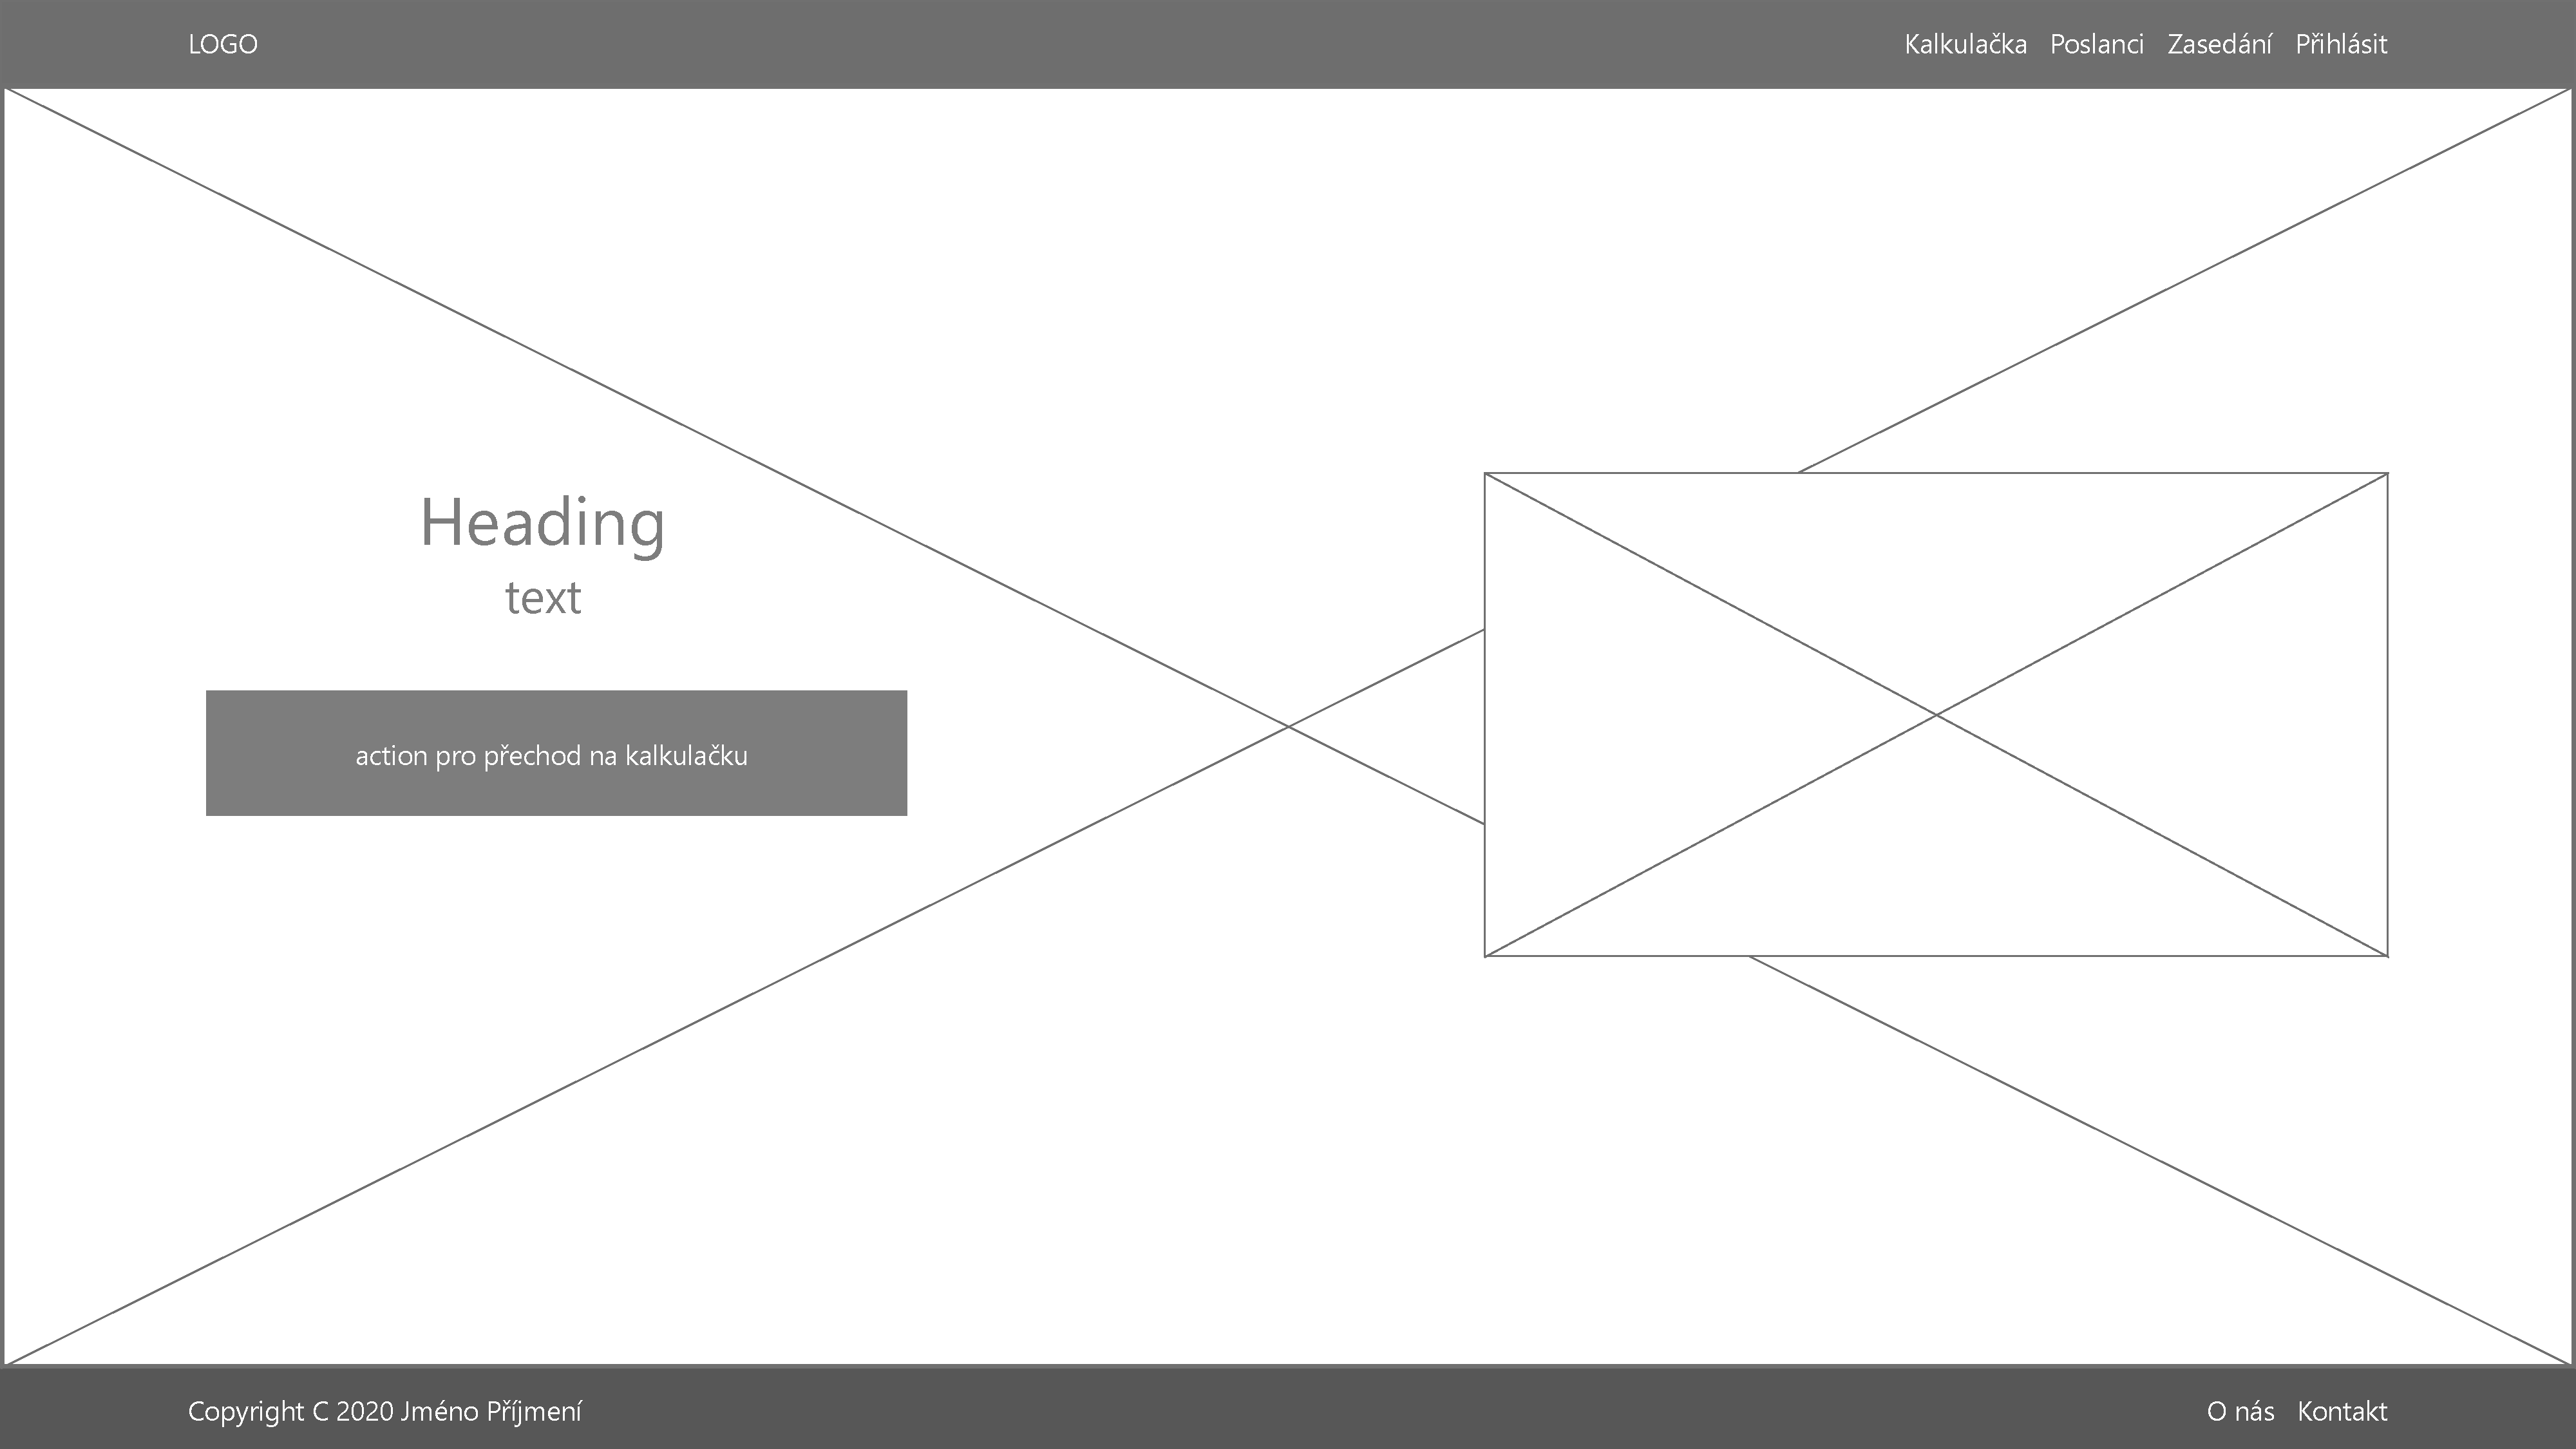
\includegraphics[width=0.8\textwidth]{obrazky-figures/wireframe-homepage.pdf}
    \caption{Drátěný model úvodní strany aplikace}
    \label{fig:wireframe-homepage}
\end{figure}



\section{Uživatelské rozhraní}
Při návrhu uživatelského rozhraní je obecně třeba dodržovat základy UX\footnote{UX: user experience} (česky \texttt{uživatelská zkušenost}) a UI\footnote{UI: user interface} (česky \texttt{uživatelské rozhraní}) designu. Tyto dva pojmy se v stále častěji zmiňují při tvorbě webových stránek a aplikací, nicméně nezřídka dochází k jejich zaměňování. 
\par UX design řeší, jakým způsobem bude uživatel s produktem pracovat. Tím obecně nemusí být myšlena jen digitální aplikace, ale může se jednat také o nějakou fyzickou věc, či službu. O cokoliv co může uživatel nějakým způsobem zažít. Do UX designu patří například drátový model, viz sekce \ref{section:wireframe}
\par Pokud jde o UI, tak na rozdíl od UX se jedná již o čistě digitální pojem. Uživatelské rozhraní je, zjednodušeně řečeno, místo, na kterém uživatel může komunikovat s aplikací. UI zahrnuje celkový vzhled, interaktivitu a intuitivnost aplikace a také celkový uživatelský pocit z používání. V současné době se zde řadí také responsivita.

\subsection{Postup při návrhu uživatelského rozhraní}
Jako první bylo třeba vypracovat základní strukturu webu se všemi prvky. K tomu posloužil již zmiňovaný drátový model. Tento byl po vytvoření prezentován nezainteresovaným lidem v roli uživatelů, aby byla získána zpětná vazba. Na jejím základě došlo k několika úpravám.
\par Jako další krok bylo potřeba vymyslet název a z něj vycházející logo celé aplikace. Jelikož smyslem celé práce je poskytnout lidem radu, čili učinit je chytřejšími (chytrý je anglicky \texttt{smart}), a následně jim díky tomu ulehčit výběr při volbě (anglicky \texttt{vote}), nabízelo se spojení právě těchto dvou slov. Původní volba byla SmartVote, nicméně po kontrole dostupnosti domény byla zvolena prohozená verze, čili VoteSmart, nebo-li česky \texttt{Volte chytře}. Samotné logo bylo následně vytvořeno ve webové aplikaci freelogodesign.org\footnote{freelogodesign.org: \url{https://www.freelogodesign.org/}}. Je tvořeno jménem webu a symbolem zaškrtávacího políčka, symbolizujícím hlavní účel webu - volbu.
\par Následuje výběr vhodného barevného schématu. Jelikož se jedná o politicky orientovanou aplikaci pro prostředí České republiky, nabízí se použití národních barev - červené, modré a bílé. Konkrétní barevné hladiny (\#11457e pro modrou a \#d7141a pro červenou) byly převzaty z jedné z použitých grafik, konkrétně z mapy České republiky\cite{grafika-mapa}, viditelné na grafickém návrhu na úvodní straně. 
\par Jako font byl zvolen Segoe UI. Primární používané velikosti jsou 35px pro nadpisy H1, 25px pro H2 a 16px pro běžný text.
\par Samotný grafický návrh, viz příloha \todo{cislo prilohy} byl vypracováván opět v programu AdobeXD. Na obrázku \ref{fig:graphic-homepage} můžete vidět design úvodní strany. Při vytváření grafického návrhu byly použity principy responsivního designu, nicméně samotný návrh je pouze pro desktopovou\footnote{Desktopová verze je slangový výraz pro běžné obrazovky stolních počítačů, obecně s poměrem stran 16:9} verzi. 

\par Při vytváření grafické předlohy byly zjištěny určité nedostatky, na které jsem při vytváření drátového modelu nenarazil. Je tedy v některých částech odlišná. Také došlo k zásadním změnám v principu fungování aplikace oproti původnímu plánu, které v drátovém modelu nejsou zpětně reflektovány. 


\begin{figure}
    \centering
    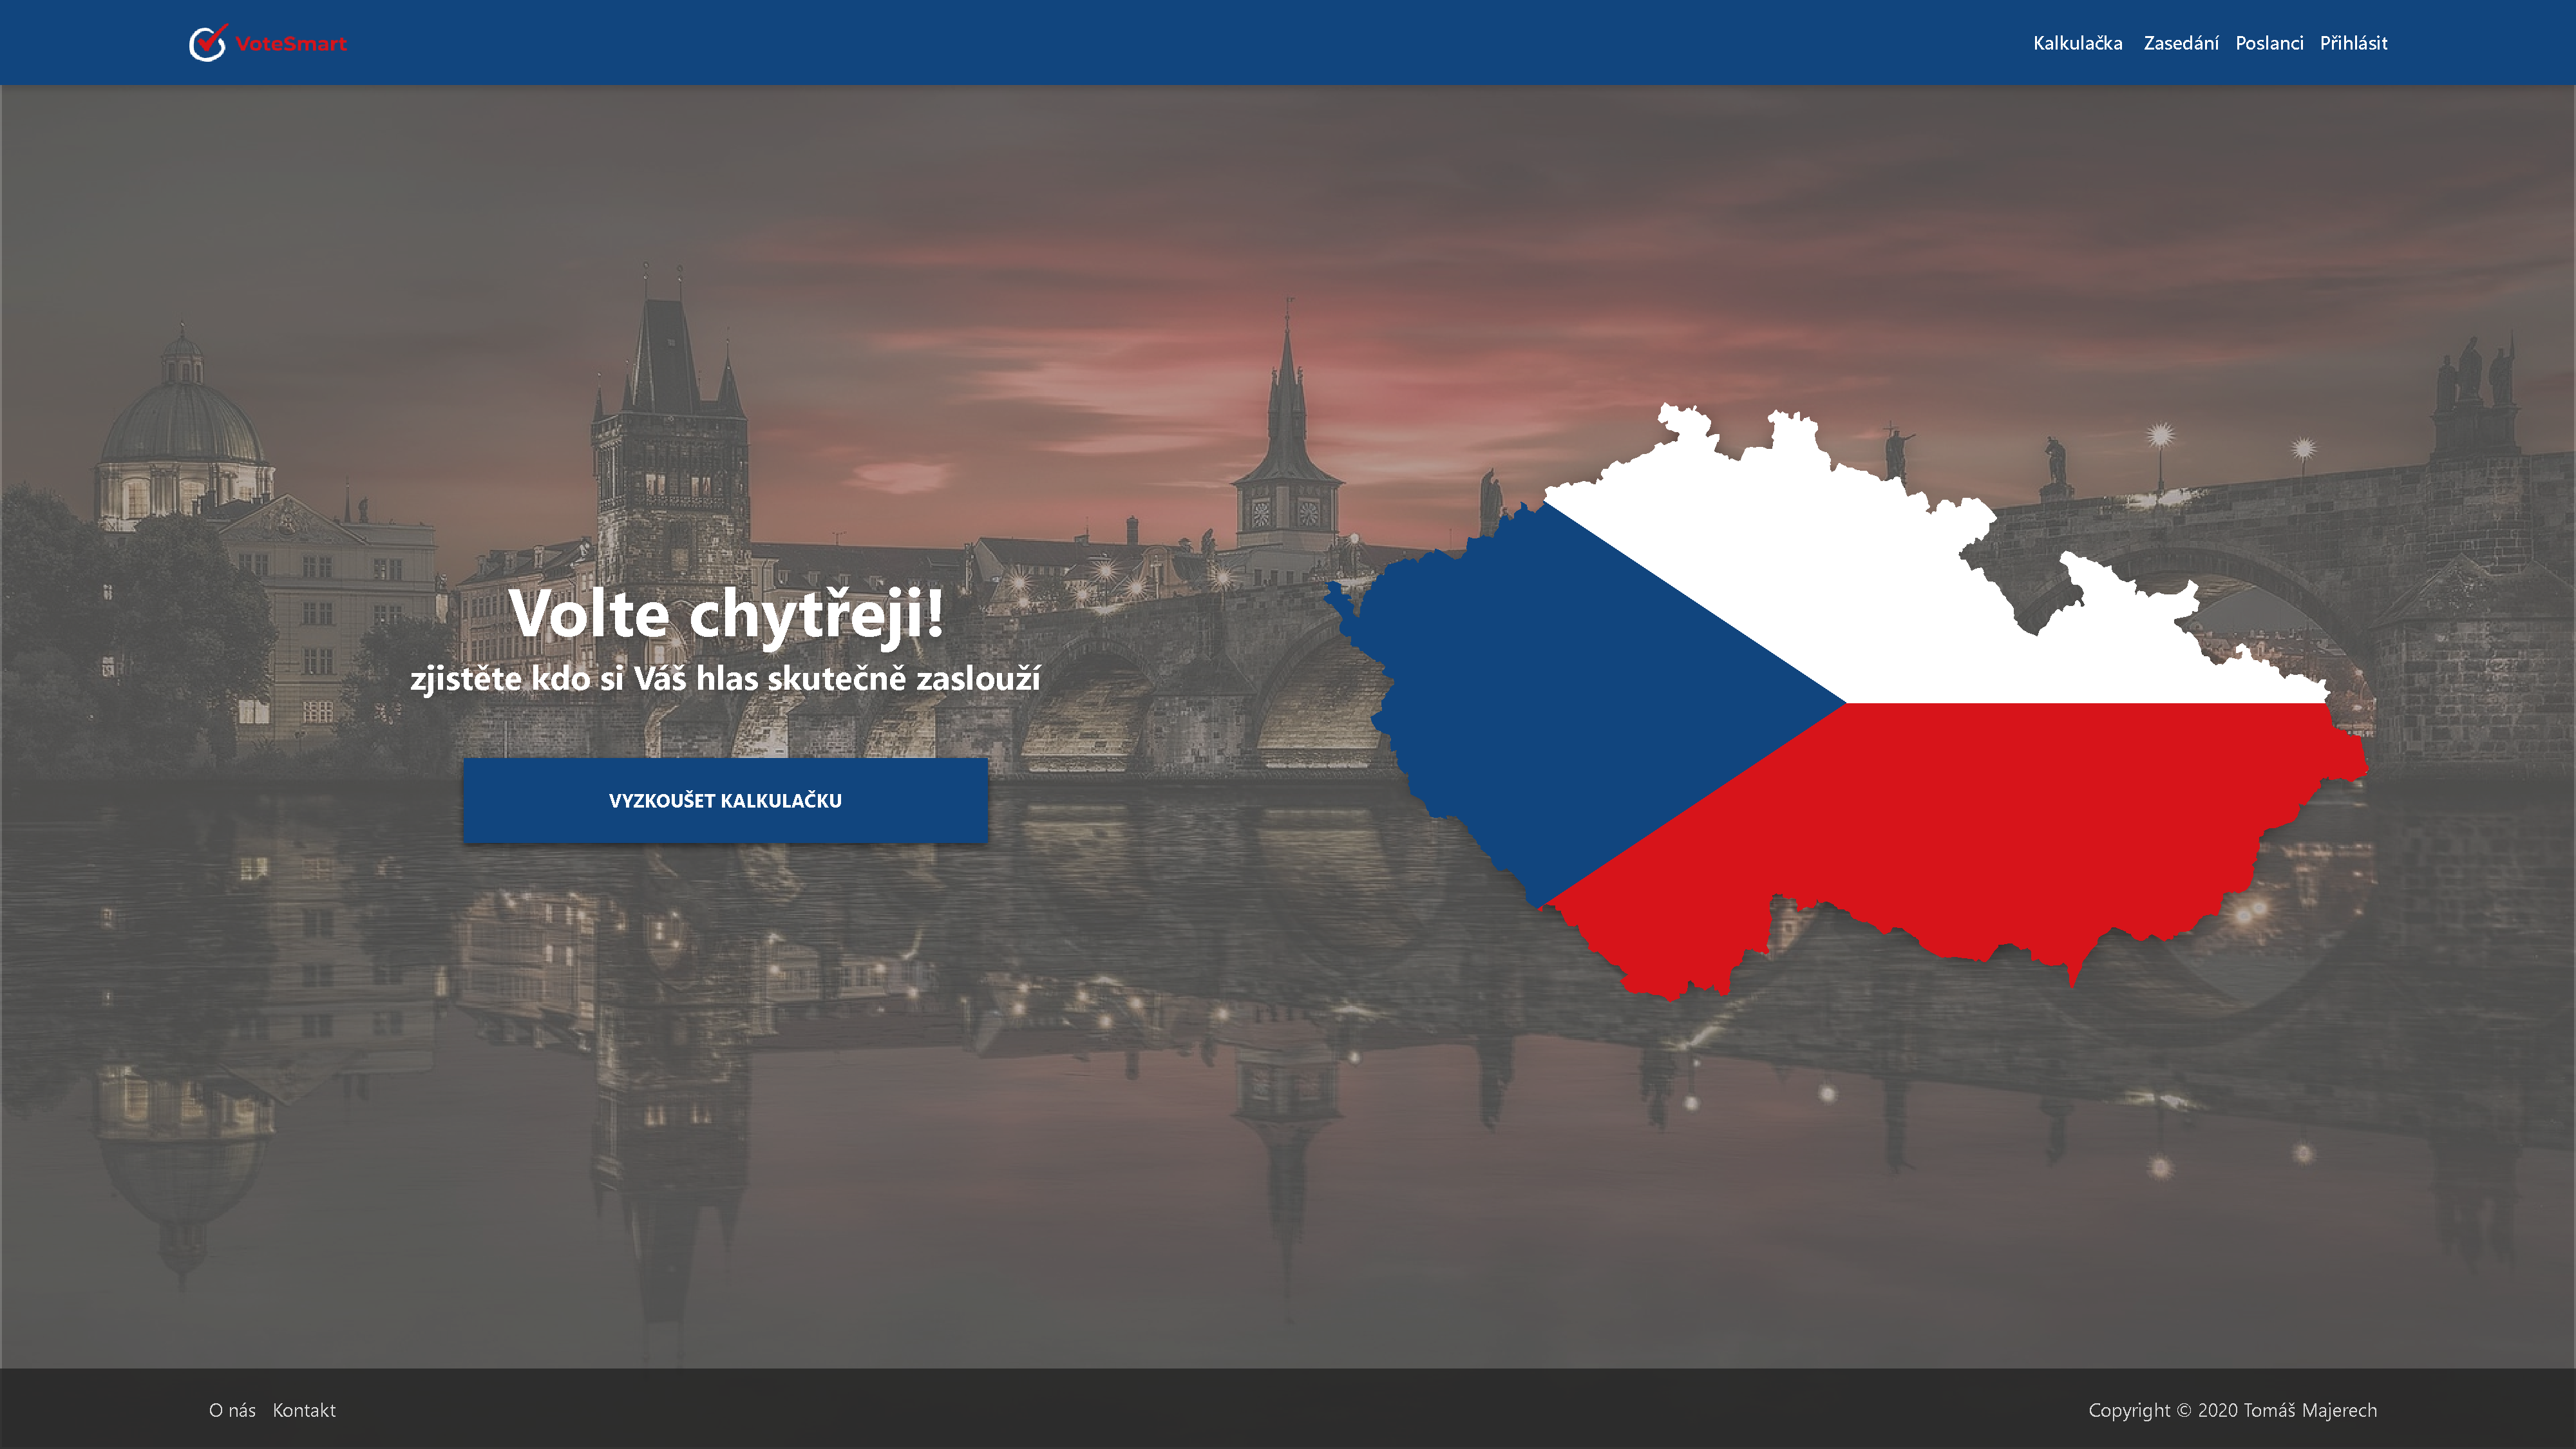
\includegraphics[width=0.8\textwidth]{obrazky-figures/Homepage.pdf}
    \caption{Grafický návrh úvodní strany aplikace}
    \label{fig:graphic-homepage}
\end{figure}

\todo{Možná rozvést jednotlivé strany?}


\section{Výběr otázek}
Jedná se o nejobtížnější a nejspíše také nejdůležitější část celé práce. Na výběru vhodných otázek totiž záleží nejenom to, nakolik dokážeme uživateli přiřadit podobnost s jednotlivými stranami a poslanci, ale také zda uživatel vůbec bude chtít aplikaci používat.\\

\par Jelikož uživatel si bude vybírat hlasování, u kterých chce sám hlasovat, je zapotřebí mu jich předložit co největší počet. Nicméně jen za aktuální volební období je těchto hlasování takřka 8000 a naprostá většina z nich nemá ve výsledku žádný vliv na to, zda bude konkrétní návrh zákona přijat či zamítnut. Proto je zde nutné zavést určitou algoritmizaci, usnadňující uživateli práci s aplikací. \\

\par Důkladným průzkumem dat, která jsou podkladem této práce, jsem došel k závěru, že na jejich základě není možné u jednotlivých hlasování strojově určit, zda konkrétní hlasování bylo rozhodující například pro přijetí návrhu a jeho posunutí do dalšího kroku, či zda šlo kupříkladu pouze o hlasování o výboru, který dostane již přijatý návrh ke zpracování. Ohledem tohoto zjištění jsem kontaktoval přímo správce dat Poslanecké sněmovny, který tento fakt potvrdil. Také však uvedl, že pro některá hlasování je možné tyto informace dohledat prostřednictví sněmovních tisků. Ty jsou součástí každého návrhu zákona a každá změna jejich stavu je zaznamenávána v tabulce \texttt{hist}.\\

\par Vzhledem k nemožnosti vyřadit irelevantní hlasování byla tedy využita pouze ta, u kterých lze pomocí tabulky \texttt{hist} určit jejich důležitost. Tím se snížil počet prezentovaný uživateli na přibližně 500 za toto volební období.\\ \todo{Doplnit konecne cislo}

\par Jelikož se stále jedná o příliš velký počet, je třeba uživateli dále usnadnit práci. Konkrétně lze například seřadit hlasování podle relevance dle algoritmického vyhodnocení jejich skóre na základě rozdílnosti hlasování jednotlivých stran. Čím větší různorodost ve hlasování napříč stranami, tím lépe z hlediska určení podobnosti uživatele se stranami a poslanci po vyhodnocení v kalkulačce. \\

\par Jakým způsobem je rozdílnost hlasování podstatná pro výpočet korelace s jednotlivými stranami je patrné například z vizualizace na obrázcích \ref{fig:analyza-rozdilne} a \ref{fig:analyza-stejne}. Zatímco z prvního grafu bychom nedokázali určit prakticky nic, jelikož takřka všichni přítomní hlasovali stejně, z toho druhého dokážeme již alespoň určitou rozdílnost vyčíst. Jen pro pořádek je však třeba zmínit, že podobnost v jednom hlasování není dostatečná a pro nějaké validní výstupy bude třeba, aby uživatel hlasoval u několika. Čím více hlasování, tím přesnější výsledky.

\begin{figure}
    \centering
    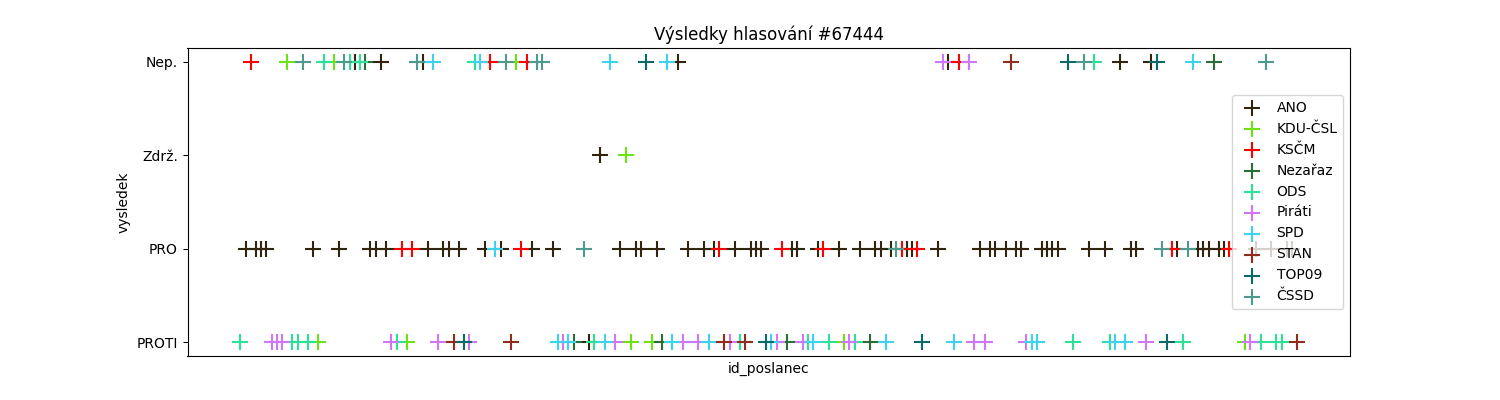
\includegraphics[width=1\textwidth]{obrazky-figures/analyza_hl_rozdilne.png}
    \caption{Vizualizace "přínosného"\ hlasování pro kalkulačku}
    \label{fig:analyza-rozdilne}
\end{figure}

\begin{figure}
    \centering
    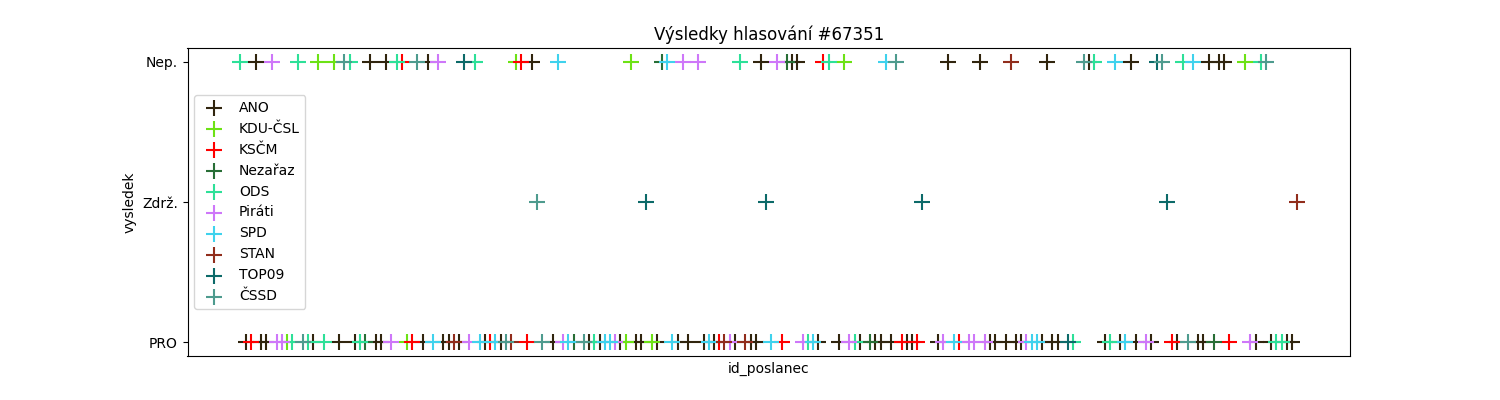
\includegraphics[width=1\textwidth]{obrazky-figures/analyza_hl_stejne.png}
    \caption{Vizualizace "nepodstatného"\ hlasování pro kalkulačku}
    \label{fig:analyza-stejne}
\end{figure}

\section{Způsob zpracování výsledků kalkulačky}
Uživatel bude "hlasovat"\ ve stejných hlasováních jako skuteční poslanci. Porovnávní proto bude probíhat komparací jeho voleb s hlasováním jednotlivých poslanců a stran u těch hlasování, kde uživatel uvedl svoji volbu. Tzn. pokud bude uživatel hlasovat například u \#67351 a \#67444, budou jeho výsledky porovnávny s výsledky poslanců pouze v těchto dvou konkrétních hlasováních. Následně se pro každého poslance vypočte procentuální shoda a výsledky se seřadí od té největší.

\par Porovnání se stranami záleží na poměru stejných odpovědí členů strany s celkovým počtem členů pro každou uživatelem odhlasovanou otázku otázku zvlášť.



\section{Výběr vhodného serveru}
Aby aplikaci mohli používat lidé, musí být umístěna na veřejně přístupném serveru. Zde máme pro web obecně 3 možnosti:
\begin{itemize}
    \item Sdílený hosting\footnote{Hosting je zažitý název pro server na kterém je aplikace, či webová stránka umístěna}\\
    Jedná se o nejlevnější a obecně nejjednodušší možnou variantu. Daň za nízkou cenu je však ve sdílení hardwaru s dalšími aplikacemi. Z toho důvodu není možné dopředu předvídat dostupné prostředky a náročnější aplikace můžou skončit chybou kvůli jejich spotřebování ostatními. Také zde uživatel ve většině případů nemá kontrolu nad nainstalovanými aplikacemi a může využívat pouze omezený počet těch předpřipravených. Je zde také bezpečnostní riziko, protože data různých aplikací jsou na stejných úložištích. Jako příklad můžeme uvést například endora.cz\footnote{endora.cz: \url{https://www.endora.cz/}}
    \item Virtuální privátní server (VPS)\\
    U tohoto typu hostování je opět hardware serveru sdílen mezi několika aplikacemi. Každý uživatel však již má k dispozici vlastní virtualizovaný systém, který je oddělen od ostatních. Poskytuje tak uživateli mnohem více prostoru pro správu i lepší zabezpečení.
    Tuto sekci můžeme dále rozdělit na spravované a nespravované virtuální privátní servery. Ty spravované opět uživateli určitým způsobem omezí kontrolu nad nainstalovanými službami, nabídnou však většinou jednoduché možnosti nasazení předem připravených prostředí pro určité specifické zaměření přes přívětivé webové rozhraní, například na cloudways.com\footnote{cloudwazys.com: \url{https://www.cloudways.com/en/}} lze jedním klikem spustit virtualizovaný server pro WordPressovou aplikaci, kdy po pár minutách uživatel dostane již plně funkční prostředí s funkční WordPress aplikací včetně databáze, cache a základních pluginů.\par
    U nespravovaných serverů má uživatel k dispozici pouze samotný server, přístup k němu a pár základních funkcí přes webové rozhraní, například možnost ho vypnout či resetovat. Všechnu další správu si uživatel musí zajistit sám - instalaci potřebných aplikací, nainstalování webového serveru, databáze, jejich propojení, nasměrování domény či vytváření subdomén, emaily a další.\\
    Podstatně dražší, než sdílená verze. Např. zmiňované cloudways.com
    \item Dedikovaný sever\\
    Nejdražší varianta. Jde o kompletně vyčleněný hardware pro použití jedním zákazníkem. Zde má zákazník plnou kontrolu nad obsahem serveru a nainstalovanými aplikacemi. Například sh.cz\footnote{sh.cz: \url{https://www.sh.cz/dedikovane-servery}}
\end{itemize}

Jelikož framework Django nespadá do úplně běžných případů užití, většina sdílených řešení ho nepodporuje. Jako východisko se tedy nabízí buď využít školní server Eva, nebo sáhnout po nějakém dražším sdíleném.
\par Zejména z důvodu výhod naprosté kontroly nad systémem a jednoduchosti nasazení jsem zvolil digitalocean.com\footnote{digitalocean.com: \url{https://www.digitalocean.com/}}, kde se dostačující sdílený VPS server dá pořídit za zhruba 5\$ měsíčně.

\section{Doména}
Jelikož přístup na web přes IP adresu není moc praktický, potřebuje server zapamatovatelnou doménu, pod kterou ho lidé budou moci vyhledat. Domény s koncovkou .cz stojí obecně zhruba 200 korun ročně a koupit ji není nic složitého. Například formulář na webu endora.cz\footnote{Endora.cz: \url{https://www.endora.cz/}} je velmi intuitivní. Zde byla také zakoupena doména použitá na vývoj této práce. Po pozdějším průzkumu bych nicméně doporučil pro umístění domén spíše wedos.cz\footnote{wedos.cz: \url{https://www.wedos.cz/}}, vzhledem k lepším možnostem pro přesměrování domény na data umístěná pod jiným správcem i k celkové roční ceně za tzv. "parkování". Domény lze však většinou kdykoliv bez poplatku přesunout mezi správci.  
\par Aby však web byl pod touto doménou dostupný, je třeba jí nejprve přidat záznam NS s odkazem na DNS servery\footnote{Dnes server je v podstatě překladač url adresy na IP adresu, viz \url{https://www.cloudflare.com/learning/dns/what-is-a-dns-server/}} zvoleného poskytovatele hostingu. Pro domény s koncovkou \texttt{.cz} je tato akce navíc specifická, protože nelze přidat jednotlivé DNS servery, nýbrž je potřeba vytvořit tzv. NSSET\footnote{Vytvoření NSSETu: \url{https://objednavka.forpsi.com/domain/cr-nsset.php}} a ten teprve přidat k záznamům pro doménu. Tím bude zajištěno, že každý dotaz hledající tuto URL adresu bude nasměrován správným směrem.

\par Aby DNS servery uměly hledanou URL adresu přeložit na IP adresu, je třeba na serveru nastavit záznamy typu A(IPV4), AAAA(IPV6) a NS. Toto nastavení lze například pro digitalocean.com vidět na obrázku \ref{fig:digitalocean-dns}.


\begin{figure}
    \centering
    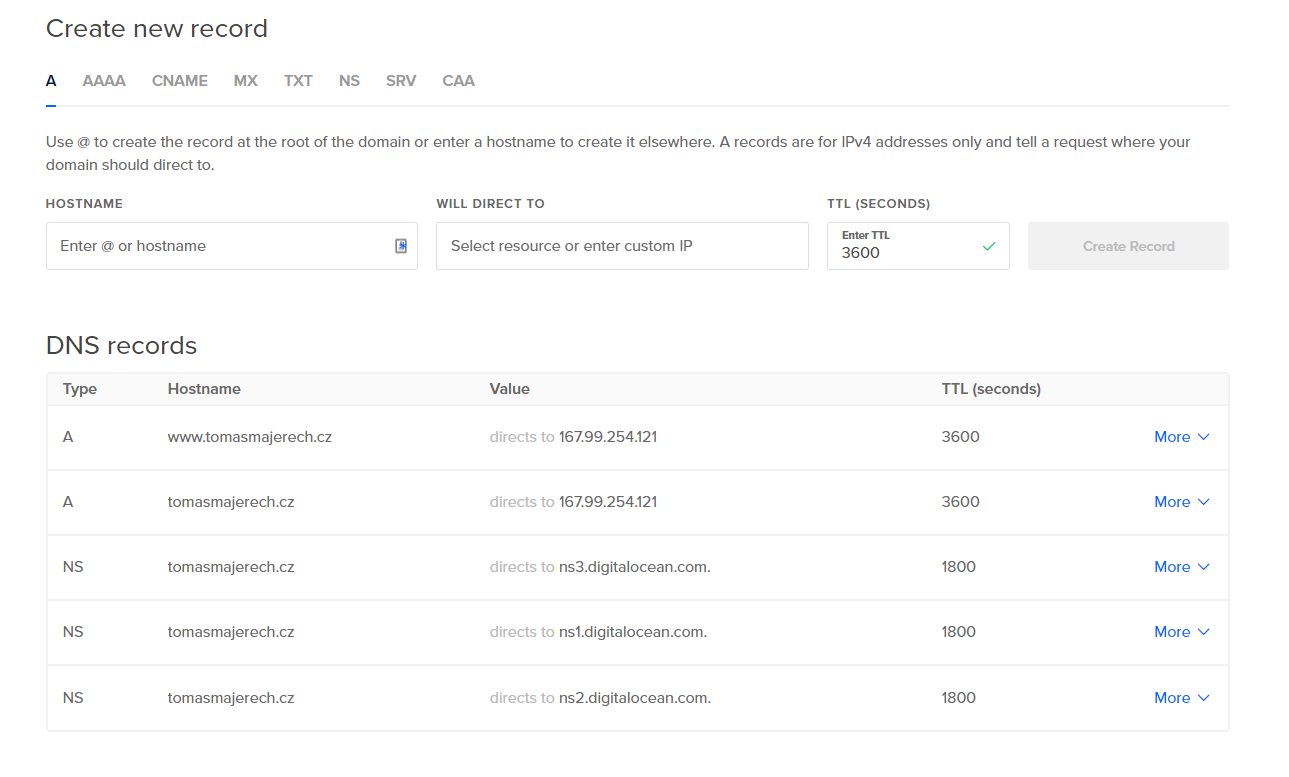
\includegraphics[width=0.9\textwidth]{obrazky-figures/digitaloceanDNSadmin.png}
    \caption{Rozhraní administrace DNS na webu digitalocean.com}
    \label{fig:digitalocean-dns}
\end{figure}

\section{?GDPR?}



\chapter{Implementace a vyhodnocení}
\label{chap:implementace}
Cílem této kapitoly je poskytnout náhled do důležitých kroků v implementaci této práce. Nejprve je popsána základní struktura aplikace, vývojové prostředí a nástroje. Následuje popis klientské části. Na ni navazuje část serverová. Kapitola je zakončena popisem databázové vrstvy.

\section{Struktura aplikace}
Jelikož základním programovacím jazykem aplikace je python, bude třeba instalovat python moduly. Ty lze samozřejmě instalovat i do celého uživatelského systému, nicméně běžně se pro jejich sdružování k jednotlivým projektům používá tzv. \texttt{virtuální prostředí}\footnote{Python Virtuální prostředí: \url{https://docs.python.org/3/library/venv.html}}. Tím docílíme oddělení python modulů využitých pro tento projekt od případných jiných verzí jinde v systému. Díky tomu odpadají problémy s možnou nekompatibilitou napříč projekty. 

\par Samotná struktura projektu je vygenerována pomocí nástroje \texttt{Cookiecutter-django}. Vygenerovaná adresářová struktura vypadá následovně.\\



\begin{minipage}[t]{.5\textwidth}
\dirtree{%
.1 volebni\_kalkulacka.
.2 .envs.
.3 .local.
.3 .production.
.2 compose.
.3 local.
.4 django.
.4 docs.
.4 node.
.3 production.
.4 django.
.4 postgres.
.4 traefik.
.2 config.
.3 settings.
.2 docs.
.2 locale.
}
\end{minipage}
\begin{minipage}[t]{.5\textwidth}
\dirtree{%
.1 .
.2 volebni\_kalkulacka.
.3 contrib.
.4 sites.
.5 migrations.
.3 static.
.4 css.
.4 fonts.
.4 images.
.5 favicons.
.4 js.
.4 sass.
.3 templates.
.4 account.
.4 pages.
.4 users.
.3 users.
.4 migrations.
.4 tests.
.3 utils.
.2 requirements.
}
\end{minipage}

\vspace{0.5cm}
tato kostra byla poté podle potřeby rozšiřována. Byl přidána samostatná podaplikace pro správu dat \texttt{dataImport} a vlastní moduly pro jednotlivé důležité části aplikace. Následuje popis jednotlivých adresářů. Postupně od vygenerovaných po vlastní.

\subsubsection{Kořenový adresář}
V kořenovém adresáři se kromě zobrazených složek nachází také další pomocné soubory. \texttt{Gulpfile.js} používaný k nastavení chování \texttt{npm} při zapnutí lokálního vývojového serveru - nastavení automatické kompilace scss do css spolu s jeho konkatenací a minifikací, automatické obnovy stránek při změně v \texttt{template} souborech, automatické doplnění nového zkompilovaného css do stránky bez nutnosti jejího nového načtení a jiné.
\par Dále také \texttt{local.yml} a \texttt{production.yml} používané ke spuštění \texttt{docker-compose} a soubor \texttt{manage.py}, který slouží jako výchozí bod pro spouštění všech příkazů týkajících se djanga. Přes něj lze spustit lokální vývojový server, vytvářet databázové migrace, migrovat databáze, používat interaktivní django shell umožňující jednoduše pracovat s django modely v konzoli a mnoho dalších věcí. 

\subsubsection{.envs}
Tato složka slouží k ukládání lokálních a produkčních proměnných. Tyto soubory se běžně nenahrávají na žádný verzovací systém a nastavují se zvlášť na každém zařízení, jelikož obsahují citlivé přihlašovací a jiné údaje.

\subsubsection{compose}
Zde jsou uloženy soubory potřebné pro docker kontejnery. Podsložky django, postgres a traefik obsahují Dockerfile, který při spuštění aplikace přes \texttt{docker-compose} nastaví příslušný kontejner.

\subsubsection{config}
Tato složka sdružuje hlavní aplikační nastavení. V souboru \texttt{base.py} se nachází všechna nastavení bez kterých by aplikace nemohla fungovat \todo{moznost rozepsat}. Soubory \texttt{local.py} a \texttt{production.py} pak slouží k upřesnění některých nastavení pro produkční a lokální nasazení. Kromě toho se zde nachází také \texttt{urls.py}, umožňující tzv. \texttt{routing}, což je vlastně určení co aplikace udělá při obdržení požadavku na určitou url adresu. Obecně se zde nastavují cesty k jednotlivým modulům aplikace do pole \texttt{urlpatterns}. Například jedna z položek
\begin{verbatim}
    path("schuze/", include("volebni_kalkulacka.schuze.urls", 
         namespace="schuze")),
\end{verbatim}

znamená, že pokud uživatel přistoupí na adresu \texttt{urlwebu.domena/schuze}, tak se všechny cesty budou hledat v souboru \texttt{urls.py} v modulu \texttt{volebni\_kalkulacka.schuze}.

\subsubsection{locale}
Tento adresář je vytvořen aby obsahoval vygenerované jazykové soubory, pokud by aplikace používala více jazyků. Cookiecuter-django v základu podporuje multijazyčnost. V této práci, jelikož je specifická jenom pro Českou Republiku, tato možnost nebyla využita, nicméně pokud by byla potřeba, stačilo by pouze nastavit proměnnou \texttt{USE\_I18N} v \texttt{base.py} na True a začít využívat tzv. \texttt{trans tagy} kolem každého textu zobrazovaného uživateli. Před nasazením aplikace do produkce by se spustil sběrač těchto textů, který by z nich vytvořil přehledný dokument. Zde by se texty ručně přeložily a následným kompilačním příkazem by se vytvořil binární soubor, ze kterého by django čerpalo při změně jazyka. Celý postup je přehledně popsán v dokumentaci\footnote{Django překlady \url{https://docs.djangoproject.com/en/3.2/topics/i18n/translation/}}.

\subsubsection{requirements}
Jelikož aplikace už v základu využívá několik python modulů, nalezneme zde jejich instalační seznam pro python instalátor \texttt{pip}. Je rozdělen stejně jako nastavení do 3 souborů - \texttt{base.txt}, \texttt{local.txt} a \texttt{production.txt}.

\subsubsection{volebni\_kalkulacka}
Hlavní aplikační složka. Zde budou umístěny všechny další navazující vytvořené moduly. V adresáři \texttt{static} se nachází všechny statické soubory, rozdělené podle typu, css, fonty, obrázky, javascript a sass před tím než se zkompiluje na css. Tyto soubory jsou po vykreslení webové stránky načítány z prohlížeče jako zdroje. Přímo z této složky je to však možné pouze v lokálním prostředí. Na produkci je nejprve nutné všechny statické soubory umístit na místo k tomu určené. Django to zvládne jedním jednoduchým příkazem\footnote{Django statické soubory: \url{https://docs.djangoproject.com/en/3.2/ref/contrib/staticfiles/}}.

\subsubsection{volebni\_kalkulacka.templates}
\par V \texttt{templates} se nachází HTML šablony používané návrhovým vzorem MVT. Jelikož šablony nejsou pouze samotné HTML, ale obsahují také Django Templating Language (django šablonovací jazyk), můžeme při vytváření šablon využívat určitý druh "dědičnosti", kdy pro základní strukturu stránky, která se bude vždy opakovat vytvoříme \texttt{base.html} soubor. Zde se bude nacházet HTML hlavička, scripty, fonty a jiné statické věci využívané napříč celým projektem. Jednotlivé stránky pak dále budou tuto základní šablonu pouze rozšiřovat. To je umožněno prostřednictví tzv. \texttt{block} (blokových) značek, kdy blok z rodičovské šablony je nahrazen blokem se stejným názvem ze šablony rozšiřující.

\subsubsection{volebni\_kalkulacka.users}
Předpřipravený modul pro správu uživatelů. Vytváří rozhraní pro registraci, správu uživatelských účtů, změnu hesla, změnu emailu a potvrzení emailu. Také jsou zde uloženy pohledy(views) pro zpracování použití kalkulačky.
 
\subsubsection{dataImport}
První z vlastních modulů. Slouží pouze k organizaci kódu potřebného pro stahování a aktualizaci dat z webu poslanecké sněmovny. 

\subsubsection{volebni\_kalkulacka.psp\_data}
Tento modul slouží výhradně k organizaci souborů týkajících se dat z poslanecké sněmovny a djanga. Všechny modely pro výchozí data jsou definovány zde. Stejně tak je zde definován script pro prvotní stažení všech dat.


\subsection{Import dat}
\label{import_dat}
Aby aplikace mohla fungovat, potřebuje mít přístup k aktuálním datům z poslanecké sněmovny. Ta jsou uložena s příponou \texttt{.unl} a jejich formát je podobný souborům \texttt{.csv}, česky zvaným \texttt{čárkou oddělené hodnoty}. S tím rozdílem, že na rozdíl od CSV obsahují oddělovač i za posledního hodnotou na řádku, což standardu CSV neodpovídá\cite{RFC4180}. Například tabulka \texttt{hl\_poslanec}, uchovávající záznamy o hlasování jednotlivých poslanců pro každé hlasování má následující formát dat\\
\\
\texttt{1539|67018|A|\\
1537|67018|A|\\
1540|67018|A|}\\
\\
kde na prvním sloupci je odkaz na unikátní identifikátor poslance v tabulce \texttt{poslanec}, ve druhém sloupci je odkaz na unikátní identifikátor hlasování v tabulce \texttt{hl\_hlasovani} a ve třetím sloupci je volba, kterou poslanec učinil. 

\par Kromě toho jsem v průběhu vývoje narazil u datových souborů na několik dalších problémů.

\begin{itemize}
    \item neexistující cizí klíče u několika tabulek\\
    např. referencovaný nadřazený typ orgánu s ID 111 v tabulce \texttt{typ\_organu}
    \item nekonzistence dat\\
    V tabulce \texttt{zarazeni} může mít sloupeček \texttt{id\_of} hodnotu cizích klíčů buď z tabulky \texttt{organy}, nebo z tabulky \texttt{funkce} v závislosti na hodnotě sloupce \texttt{cl\_funkce}.
    \item data nekorespondující k deklarovanému typu podle popisu tabulek\\
    Ve sloupcích podle popisu definovaných jako INT, či-li celočíselné, se nachází nejenom čísla ale někdy také písmena či kombinace čísel a písmen. Například v tabulce \texttt{tisky} se ve sloupci \texttt{zm\_lhuty} nachází kromě v popisu deklarovaných hodnot "1"\ a "2"\ také hodnoty "a"\ a "n".
    \item Kódování souborů nekorespondující s deklarovaným v popisu dat, ani s žádným z několika možných vyzkoušených.\\
    Například u tabulky \texttt{tisky} by stejně jako u ostatních tabulek mělo fungovat deklarované kódování \texttt{windows-1250}, nicméně při pokusu o otevření s tímto kódováním dochází k chybám. Bylo proto nutné nastavit parametr \texttt{errors='replace'}, na základě kterého dojde k nahrazení nečitelných znaků. Tyto znaky však poté byly zobrazeny na webu a podstatně zhoršovaly uživatelskou zkušenost, proto bylo třeba je nahradit zpětně zase na odpovídající české znaky.
    \item Nejednoznačnost prázdných hodnot
    V některých tabulkách je prázdné pole zaznačeno oddělovači sloupců u sebe, což odpovídá hodnotě NULL, čili žádné. Nicméně jinde jsou jako prázdné hodnoty použity mezery, či lomítka. Například v případě tabulky \texttt{osoby} a sloupce \texttt{pred} je to buď NULL, nebo mezera.
    
    
\end{itemize}

\subsubsection{Prvotní naplnění databáze}
Prvotní naplnění databáze lze provést přes příkaz
\begin{verbatim}
    python3 manage.py initial_import
\end{verbatim}
z kořenového adresáře aplikace. Jeho definice se nachází v souboru\\
\texttt{volebni\_kalkulacka.psp\_data.management.commands.initial\_import.py}. \\

\par V prvotní verzi tento script zpracovával každý nahrávaný soubor řádek po řádku a každý zvlášť vkládal po dávkách do databáze. Tímto způsobem bylo možné lépe kontrolovat jak budou data zpracována a případně opravit nalezené chyby. Nicméně po změně koncepce aplikace a nutnosti zpracovávat všechna data bez omezení na pouze poslední volební období jsem narazil na výkonnostní problémy, kdy by zpracování zhruba 17 milionů řádků databáze přestalo být realizovatelné.
Proto bylo nutné navrhnout lepší způsob.

\par Současná verze již utilizuje PostgreSQL příkaz \texttt{COPY}, díky kterému je možné zpracovávat celé soubory najednou\cite{psql-copy}, velmi zásadně zvýšilo rychlost, jakou jsou data do databáze nahrána. Bohužel v důsledku toho již není možné průběžně data upravovat. Navíc je třeba převést unl formát na csv.

\par Samotný script tedy funguje následovně. Nejprve dynamicky získáme odkazy všech stažitelných zip souborů na stránce s daty. Tímto zajistíme automatické přidání nových volebních období bez nutnosti úpravy kódu. Následně jsou všechny staženy a rozbaleny. 
\par Některé soubory zůstávají neměnné napříč všemi volebními obdobími. Jejich názvy jsou uloženy v souboru s konstantami v konstantě s názvem \texttt{INITIAL\_FILE\_NAMES} s datovým typem \texttt{dict} neboli česky slovník, kde je navázán název databázové tabulky na odpovídající jméno staženého souboru. Přes tyto dvojice (tabulka:soubor) je iterováno hned 2x. Poprvé je to kvůli již zmiňovanému unl formátu, konkrétně poslednímu oddělovači. Tento musí být odstraněn, jelikož příkaz COPY očekává, že za každým oddělovačem v souboru se nachází nový sloupec. Nahrávaný soubor je tedy otevřen a do nového souboru s příponou \texttt{\_formatted} je uložen jeho obsah již bez tohoto nezbedného znaku.
\par Druhá iterace nejprve provede nad danou tabulkou příkaz \texttt{TRUNCATE RESTART IDENTITY}, který z ní smaže všechna data a vynuluje čítač řádků pro tabulky bez primárního klíče\cite{psql-truncate}. Dále získá hlavičky souboru, respektive tabulky, z konstanty \texttt{TABLE\_HEADERS}, což je opět slovník dvojic, nyní ve tvaru (tabulka:pole názvů hlaviček). Následuje vypnutí databázových spouštěčů (anglicky trigger), aby bylo možné nahrát i data s nekonzistentními hodnotami, nahrání dat a opětovné zapnutí spouštěčů. 

\par Pro soubory s hlasováním je postup stejný, s tím rozdílem, že se budou objevovat nové názvy souborů pro nová volební období. Názvy jsou proto v této fázi vybírány dynamicky ze stažených souborů a všechny se nahrávají do jedné tabulky. Stejný princip je uplatněn jak pro tabulky \texttt{hl\_poslanec} tak \texttt{hl\_hlasovani}.\\

\par Po uložení všech potřebných dat jsou odstraněna zmatečná hlasování.\\ 

\par Dalším krokem je výpočet ohodnocení jednotlivých důležitých hlasování - těch která mají zásadní vliv na další existenci návrhů zákona. Tato funkce je jedna z nejpodstatnějších částí aplikace, jelikož je důležité uživateli hned zpočátku předložit v kalkulačce ty nejzajímavější možnosti. Samotný kód realizující tuto operaci se nachází v metodě \texttt{calculateHlasovaniRatings} třídy \texttt{DbManager} zajišťující práci s databází pro import dat, umístěné v souboru \texttt{volebni\_kalkulacka.dataImport.Logic.DbManager.py}. 
\par Nejdříve potřebujeme získat všechna důležitá hlasování za poslední dvě volební období. K tomuto účelu využívám SQL dotaz propojující tabulku \texttt{hl\_hlasovani} s tabulkou \texttt{hist}, kde hledáme pouze hlasování spadající do orgánů značících poslední 2 volební období:

\begin{lstlisting}[language=SQL, caption={SQL dotaz na všechna podstatná hlasování za poslední 2 volební období}, label=code:sql-dve-obdobi]
SELECT * 
FROM 
    psp_data_hl_hlasovani as hh

    INNER JOIN psp_data_hist as h
    ON h.id_hlas = hh.id_hlasovani

WHERE 
    hh.id_organ IN (
        --last 2 election periods
        select 
            id_organ from psp_data_organy 
        where 
            organ_id_organ is null
            and id_typ_organu = 11 --poslanecka snemovna
        union
        select id_organ-1 from psp_data_organy 
        where 
            organ_id_organ is null
            and id_typ_organu = 11 --poslanecka snemovna
    )
\end{lstlisting}

Následně již v pythonu provedeme nad získanými daty cyklus, kdy pro každé z hlasování pokládáme další dotaz do databáze. Tentokrát hledáme dvojici (zkratka, vysledek), kde zkratka je zkratka strany a vysledek je hlasováni poslance. Jedna dvojice za každého poslance zúčastněného v konkrétním hlasování. \todo{prostor pro rozsireni}\\
\begin{lstlisting}[language=SQL, caption={SQL dotaz na získání dvojic zkratka, výsledek pro zadané hlasování}, label=code:sql-zkratka-vysledek]
SELECT 
    zkratka,vysledek
FROM 
    psp_data_hl_poslanec AS hp 

    INNER JOIN psp_data_poslanec AS p 
    ON hp.id_poslanec = p.id_poslanec 
    
    INNER JOIN psp_data_zarazeni AS z
    ON p.id_osoba = z.id_osoba
    
    INNER JOIN psp_data_organy as o
    ON z.id_of = o.id_organ
    
    INNER JOIN psp_data_osoby as os
    ON os.id_osoba = p.id_osoba
WHERE 
    hp.id_hlasovani = {hlasovani['id_hlasovani']}
    AND z.cl_funkce = 0 --clenstvi
    AND o.organ_id_organ = {hlasovani['id_organ']} --ID election period 
    AND o.id_typ_organu = 1 --Klub
    AND ( --either membership is active (null) 
        --or membership ended together with election period
        TO_DATE(z.do_o, 'YYYY-MM-DD') = TO_DATE(o.do_organ,'DD.MM.YYYY')
        OR 
        z.do_o IS null
    )
\end{lstlisting}

Výsledek databázového dotazu je načten do knihovny Pandas, což je rychlý, výkonný, flexibilní a jednoduše ovladatelný open-source nástroj pro manipulaci s daty a jejich analýzu\cite{pandas}. Zde je opět cyklus, v tomto případě pro každou ze zúčastněných stran v hlasování. Výpočet ohodnocení hlasování se dá popsat sumou
\begin{equation}
    \sum_{i=1}^N \Big(1-\Big|\frac{pocet\_pro_i}{pocet\_clenu_i}-\frac{pocet\_proti_i}{pocet\_clenu_i}\Big|\Big) * \frac{pocet\_clenu_i}{pocet\_vsech\_zucastnenych} * 100
\end{equation}

kde \texttt{N} je celkový počet stran, \texttt{i} odpovídá jedné ze stran přes kterou cyklus zrovna prochází, \texttt{pocet\_pro} je počet poslanců ve straně hlasujících pro přijetí, \texttt{pocet\_proti} je počet poslanců ve straně hlasujících pro zamítnutí, \texttt{pocet\_clenu} je celkový počet přítomných členů strany hlasujících pro přijetí/zamítnutí a \texttt{pocet\_vsech\_zucastnenych} je celkový počet členů všech stran přítomných na tomto hlasování.

\par Cílem tohoto hodnocení je nalézt ta hlasování, kde poslanci jednotlivých stran hlasovali nejvíce rozdílně. Či-li kde je nejmenší rozdíl mezi hlasy pro a proti uvnitř jednotlivých stran. Tento rozdíl dále násobíme poměrem velikosti strany k celkovému počtu členů parlamentu, aby se přizpůsobila váha jednotlivých stran k jejich velikosti.  

\par Výsledek hodnocení poté uložíme spolu s číslem hlasování do tabulky \texttt{hl\_hlasovani\_rating}. Při výpisu uživateli poté řadíme hlasování od těch s největším ohodnocením.\\

\par Nakonec je spuštěna funkce na nahrazení nevalidních znaků popsaných v problémech s daty na začátku kapitoly \ref{import_dat}. 

\subsection{Kalkulačka shod}
U každého hlasování může uživatel sám hlasovat. K tomuto účelu slouží malý modul po straně, kde si uživatel může vybrat ze tří možností. Pro, proti a zdržet se. Může také svoji volbu zrušit. Vše je patrné z obrázku \ref{fig:aplikace-hlasovani}.

\begin{figure}
    \centering
    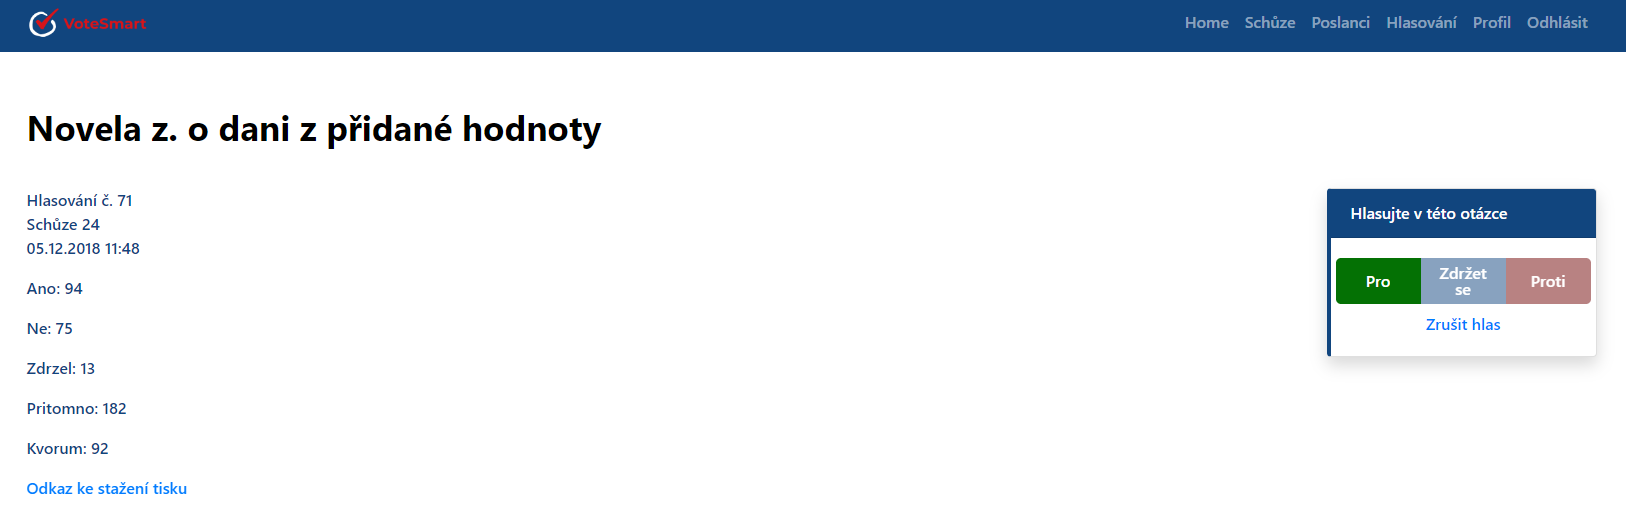
\includegraphics[width=1\textwidth]{obrazky-figures/aplikace-hlasovani.png}
    \caption{Rozhraní pro uživatelské hlasování}
    \label{fig:aplikace-hlasovani}
\end{figure}

\par Své výsledky si uživatel může zobrazit ve svém uživatelském profilu viz obrázek \ref{aplikace-kalkulacka}. Jelikož uživatel může hlasovat napříč několika volebními obdobími, byly výsledky rozděleny podle toho kam patří. Uživatel tedy má jeden výsledek pro každé období zvlášť. 

\begin{figure}[H]
    \centering
    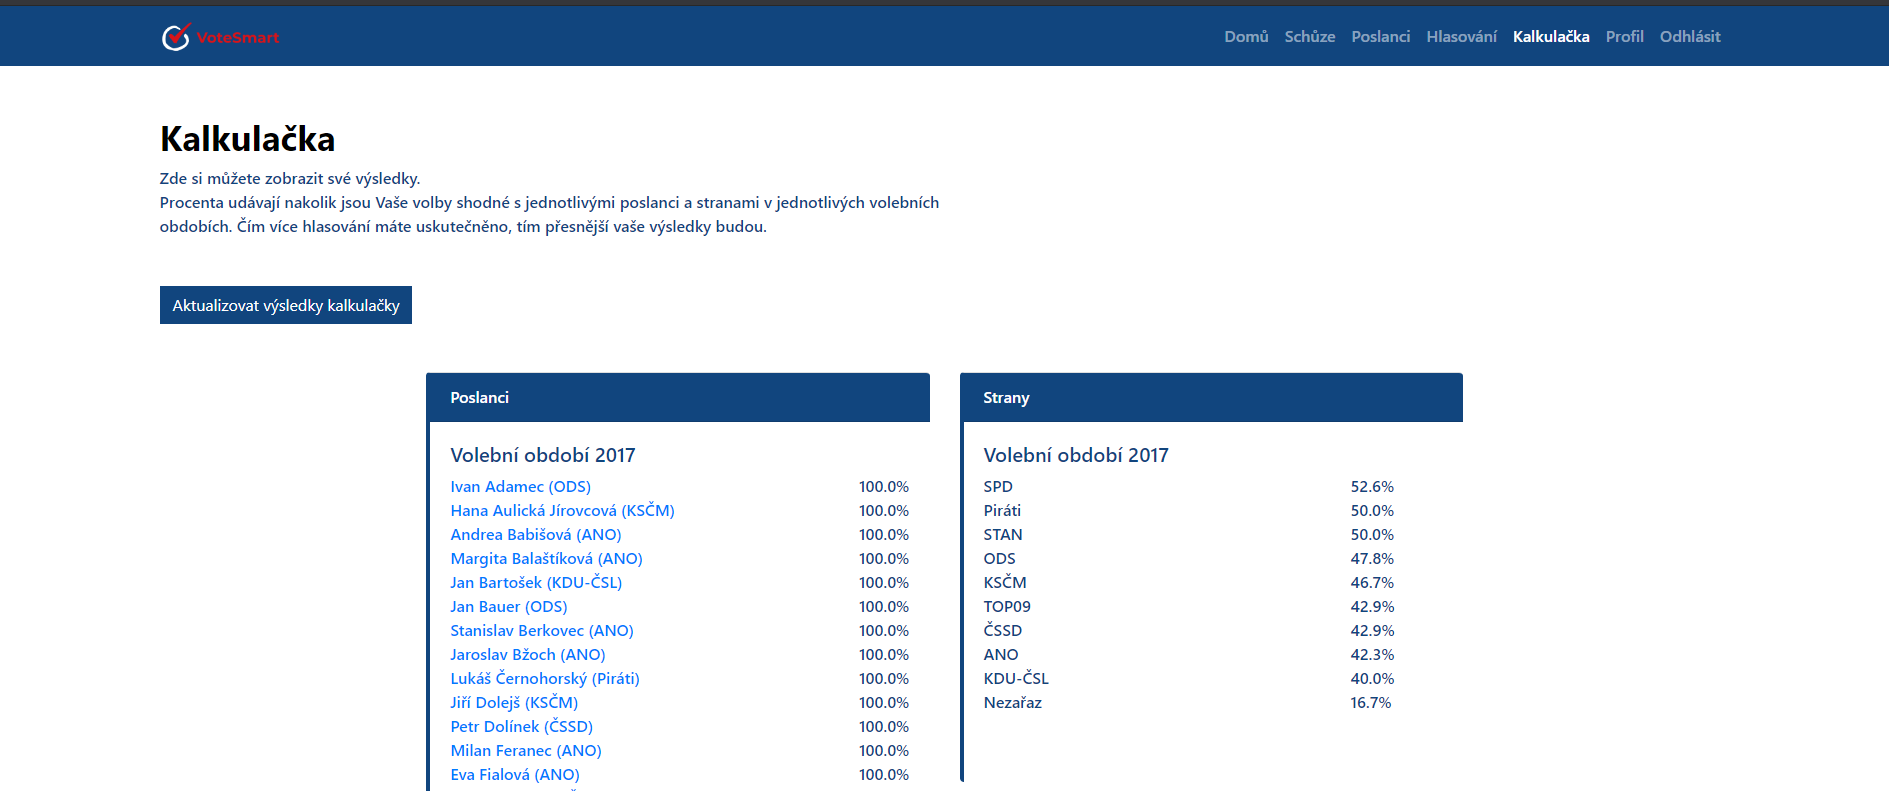
\includegraphics[width=0.7\textwidth]{obrazky-figures/aplikace-kalkulacka.png}
    \caption{Zobrazení výsledků kalkulačky v uživatelském profilu}
    \label{fig:aplikace-kalkulacka}
\end{figure}

\par Vyhodnocení shod probíhá v cyklu pro všechna období. Pro shodu s poslanci je použit SQL dotaz, kteý nejprve vyhledá všechny dvojice \texttt{matches}, \texttt{id\_poslanec}, kde id\_poslanec je unikátní identifikátor poslance a sloupeček matches uchovává počet jeho shodných hlasování s uživatelem. Tyto informace jsou poté ve druhém databázovém dotazu spojeny do jedné tabulky spolu s daty o jednotlivých poslancích a jejich zařazení ve stranách v zadaném volebním období. Výsledkem je pole trojic \texttt{match\_ratio}, \texttt{id\_poslanec}, \texttt{zkratka}, kde match\_ratio je poměr shod poslance s uživatelem a zkratka je zkratka jeho strany, který je poté zobrazen v kalkulačce.

\begin{lstlisting}[language=SQL, caption={SQL dotaz na vyhledání shod uživatele s poslanci}, label=code:sql-shoda-poslanci]

DROP TABLE IF EXISTS t1;
CREATE TEMP TABLE t1 AS   
    SELECT count(*) AS matches, id_poslanec 
    FROM psp_data_hl_poslanec
    WHERE (id_hlasovani, REPLACE(REPLACE(vysledek, 'N', 'B'),'C', 'K')) IN %s
    GROUP BY id_poslanec 
    ORDER BY matches DESC;
    
SELECT (cast(t1.matches as decimal(7,2))/%s)*100 AS match_ratio, 
    t1.id_poslanec, o.zkratka, os.pred, os.jmeno, os.prijmeni, os.za
FROM t1
    INNER JOIN psp_data_poslanec AS p
    ON p.id_poslanec = t1.id_poslanec

    INNER JOIN psp_data_osoby AS os
    ON p.id_osoba = os.id_osoba

    INNER JOIN psp_data_zarazeni AS z 
    ON p.id_osoba = z.id_osoba

    INNER JOIN psp_data_organy as o
    ON z.id_of = o.id_organ
WHERE z.cl_funkce = 0
    AND o.organ_id_organ = {period_id}
    AND o.id_typ_organu = 1
    AND (
        TO_DATE(z.do_o, 'YYYY-MM-DD') = TO_DATE(o.do_organ,'DD.MM.YYYY')
        OR 
        z.do_o IS null
    )
\end{lstlisting}

\par Shody se stranami jsou počítány obdobně. Nejprve jsou získány počty poslanců ve všech stranách v procházeném volebním období. Dále počet hlasů shodných s uživatelem pro každou stranu. V posledním kroku se tyto dvě informace spojí a na výstupu je opět pole, tentokráte dvojic \texttt{match\_ration}, \texttt{zkratka}, kde match\_ration je procentuálně vyjádřena shoda uživatelských voleb a průměrné shody na jednoho poslance ve straně.

\begin{lstlisting}[language=SQL, caption={SQL dotaz na vyhledání shod uživatele se stranami}, label=code:sql-shoda-strany]
--get members count in party
DROP TABLE IF EXISTS tP1;
CREATE TEMP TABLE tP1 AS
    SELECT 
        COUNT(*) AS members_count, o.zkratka FROM psp_data_osoby AS os
        INNER JOIN psp_data_zarazeni AS z 
        ON os.id_osoba = z.id_osoba

        INNER JOIN psp_data_organy AS o
        ON z.id_of = o.id_organ
    WHERE 
        z.cl_funkce = 0
        and o.organ_id_organ = {period_id}
        and o.id_typ_organu = 1
        and (
            TO_DATE(z.do_o, 'YYYY-MM-DD') = TO_DATE(o.do_organ,'DD.MM.YYYY')
            OR 
            z.do_o IS null
        )
    GROUP BY o.zkratka;

DROP TABLE IF EXISTS tP2;
CREATE TEMP TABLE tP2 AS
    SELECT 
        count(*) AS party_total_matches, 
        o.zkratka FROM psp_data_hl_poslanec as hlp
        
        INNER JOIN psp_data_poslanec AS p
        ON p.id_poslanec = hlp.id_poslanec

        INNER JOIN psp_data_osoby AS os
        ON p.id_poslanec = os.id_osoba

        INNER JOIN psp_data_zarazeni AS z 
        ON p.id_osoba = z.id_osoba

        INNER JOIN psp_data_organy as o
        ON z.id_of = o.id_organ

    --need to replace characters because they use multiple with same meaning
    WHERE 
        (id_hlasovani, REPLACE(REPLACE(vysledek, 'N', 'B'),'C', 'K')) IN %s
        and z.cl_funkce = 0
        and o.organ_id_organ = {period_id}
        and o.id_typ_organu = 1
    GROUP BY o.zkratka;

SELECT 
    ((CAST(tP2.party_total_matches as decimal(7,2))/{answers_count})
    /tP1.members_count)*100 AS match_ratio, tP1.zkratka 
FROM tP2
    INNER JOIN tP1
    ON tP1.zkratka = tP2.zkratka
ORDER 
    BY match_ratio DESC
\end{lstlisting}

\chapter{Testování}
\label{chap:testovani}




\chapter{Závěr (1 strana)}
\label{chap:zaver}
  \fi
  
  % Kompilace po částech (viz výše, nutno odkomentovat)
  % Compilation piecewise (see above, it is necessary to uncomment it)
  %\subfile{projekt-01-uvod-introduction}
  % ...
  %\subfile{chapters/projekt-05-conclusion}


  % Pouzita literatura / Bibliography
  % ----------------------------------------------
\ifslovak
  \makeatletter
  \def\@openbib@code{\addcontentsline{toc}{chapter}{Literatúra}}
  \makeatother
  \bibliographystyle{bib-styles/Pysny/skplain}
\else
  \ifczech
    \makeatletter
    \def\@openbib@code{\addcontentsline{toc}{chapter}{Literatura}}
    \makeatother
    \bibliographystyle{bib-styles/Pysny/czplain}
  \else 
    \makeatletter
    \def\@openbib@code{\addcontentsline{toc}{chapter}{Bibliography}}
    \makeatother
    \bibliographystyle{bib-styles/Pysny/enplain}
  %  \bibliographystyle{alpha}
  \fi
\fi
  \begin{flushleft}
  \bibliography{projekt-20-literatura-bibliography}
  \end{flushleft}

  % vynechani stranky v oboustrannem rezimu
  % Skip the page in the two-sided mode
  \iftwoside
    \cleardoublepage
  \fi

  % Prilohy / Appendices
  % ---------------------------------------------
  \appendix
\ifczech
  \renewcommand{\appendixpagename}{Přílohy}
  \renewcommand{\appendixtocname}{Přílohy}
  \renewcommand{\appendixname}{Příloha}
\fi
\ifslovak
  \renewcommand{\appendixpagename}{Prílohy}
  \renewcommand{\appendixtocname}{Prílohy}
  \renewcommand{\appendixname}{Príloha}
\fi
%  \appendixpage

% vynechani stranky v oboustrannem rezimu
% Skip the page in the two-sided mode
%\iftwoside
%  \cleardoublepage
%\fi
  
\ifslovak
%  \section*{Zoznam príloh}
%  \addcontentsline{toc}{section}{Zoznam príloh}
\else
  \ifczech
%    \section*{Seznam příloh}
%    \addcontentsline{toc}{section}{Seznam příloh}
  \else
%    \section*{List of Appendices}
%    \addcontentsline{toc}{section}{List of Appendices}
  \fi
\fi
  \startcontents[chapters]
  \setlength{\parskip}{0pt} 
  % seznam příloh / list of appendices
  % \printcontents[chapters]{l}{0}{\setcounter{tocdepth}{2}}
  
  \ifODSAZ
    \setlength{\parskip}{0.5\bigskipamount}
  \else
    \setlength{\parskip}{0pt}
  \fi
  
  % vynechani stranky v oboustrannem rezimu
  \iftwoside
    \cleardoublepage
  \fi
  
  % Přílohy / Appendices
  \ifenglish
    \input{projekt-30-prilohy-appendices-en}
  \else
    \chapter{Instalační manuál}
\label{append:instalace}
\section{Lokální vývojové prostředí}
\label{append:instalace-local}

\section{Produkční prostředí}
\label{append:instalace-production}
  \fi
  
  % Kompilace po částech (viz výše, nutno odkomentovat)
  % Compilation piecewise (see above, it is necessary to uncomment it)
  %\subfile{projekt-30-prilohy-appendices}
  
\end{document}
